\chapter{Surface Generation}
%

%%%%%%%%%%%%%%%%%%%%%%%%%%%%%%%%%%%%%%%%%%%%%%%
%%%%%%%%%%%%%%%%%%%%%%%%%%%%%%%%%%%%%%%%%%%%%%%
\section{Surface Generation Approaches}
\label{Surface Generation Approaches}

%%%%%%%%%%%%%%%%%%%%%%%%%%%%%%%%%%%%%%%%%%%%%%%
%%%%%%%%%%%%%%%%%%%%%%%%%%%%%%%%%%%%%%%%%%%%%%%
\section{Point Cloud Generation}
\label{Point Cloud Generation}

%%%%%%%%%%%%%%%%%%%%%%%%%%%%%%%%%%%%%%%%%%%%%%%
%%%%%%%%%%%%%%%%%%%%%%%%%%%%%%%%%%%%%%%%%%%%%%%
\section{Surface Reconstruction}
\label{Surface Reconstruction}

\subsection{Surface Reconstruction Approaches}
\label{Surface Reconstruction Approaches}

\subsection{Voronoi-Based Surface Reconstruction}
\label{Voronoi-Based Surface Reconstruction}

\begin{figure}[ht]
\centering
\subfigure[]{%
		
\includegraphics[scale=0.57]{media/2-shabaka/1-vor/dem1.png}
\label{fig:vor1}}
\subfigure[]{%
		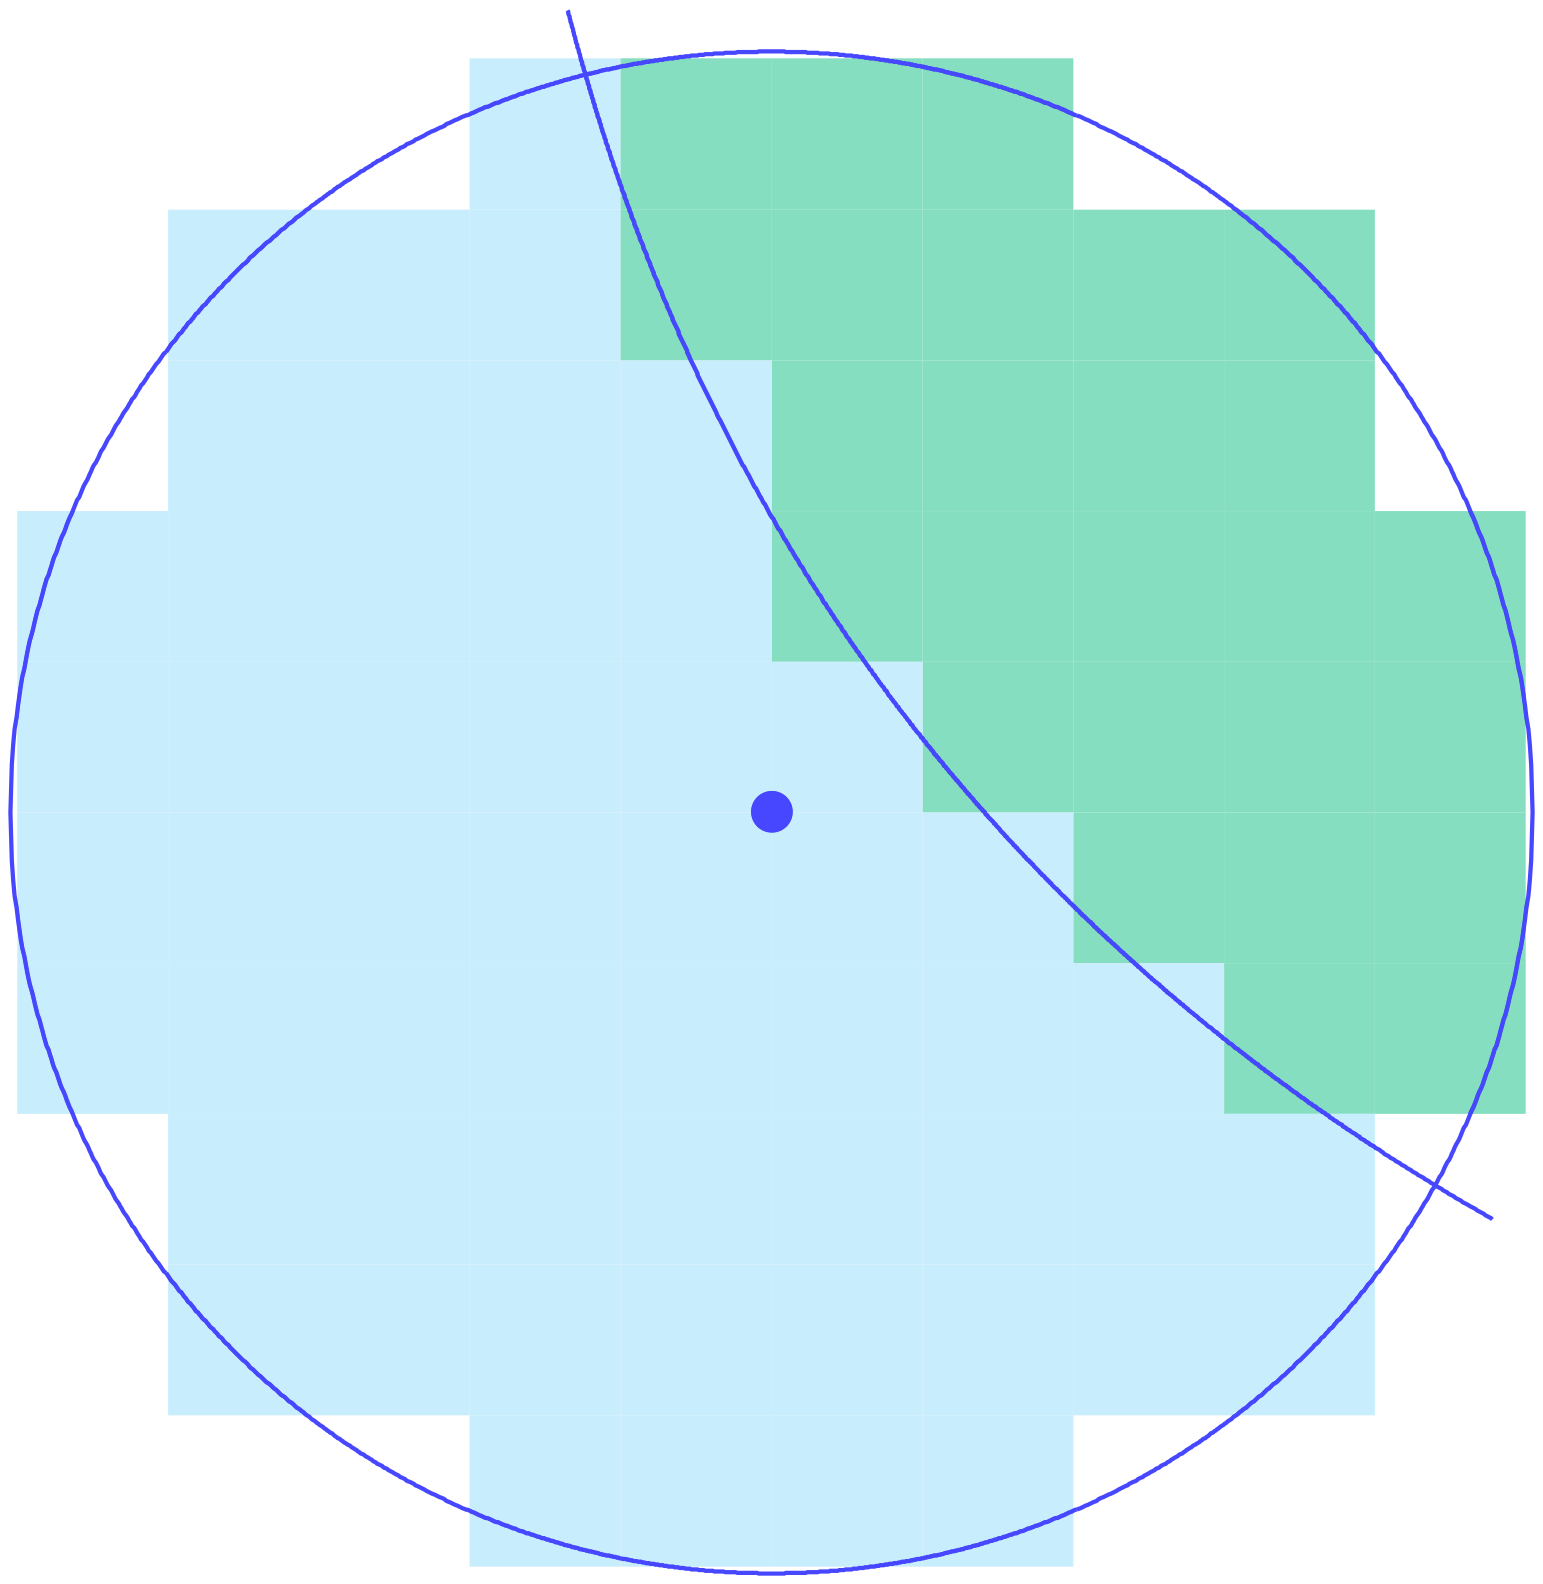
\includegraphics[scale=0.57]{media/2-shabaka/1-vor/dem2.png}
\label{fig:vor2}}
\subfigure[]{%
		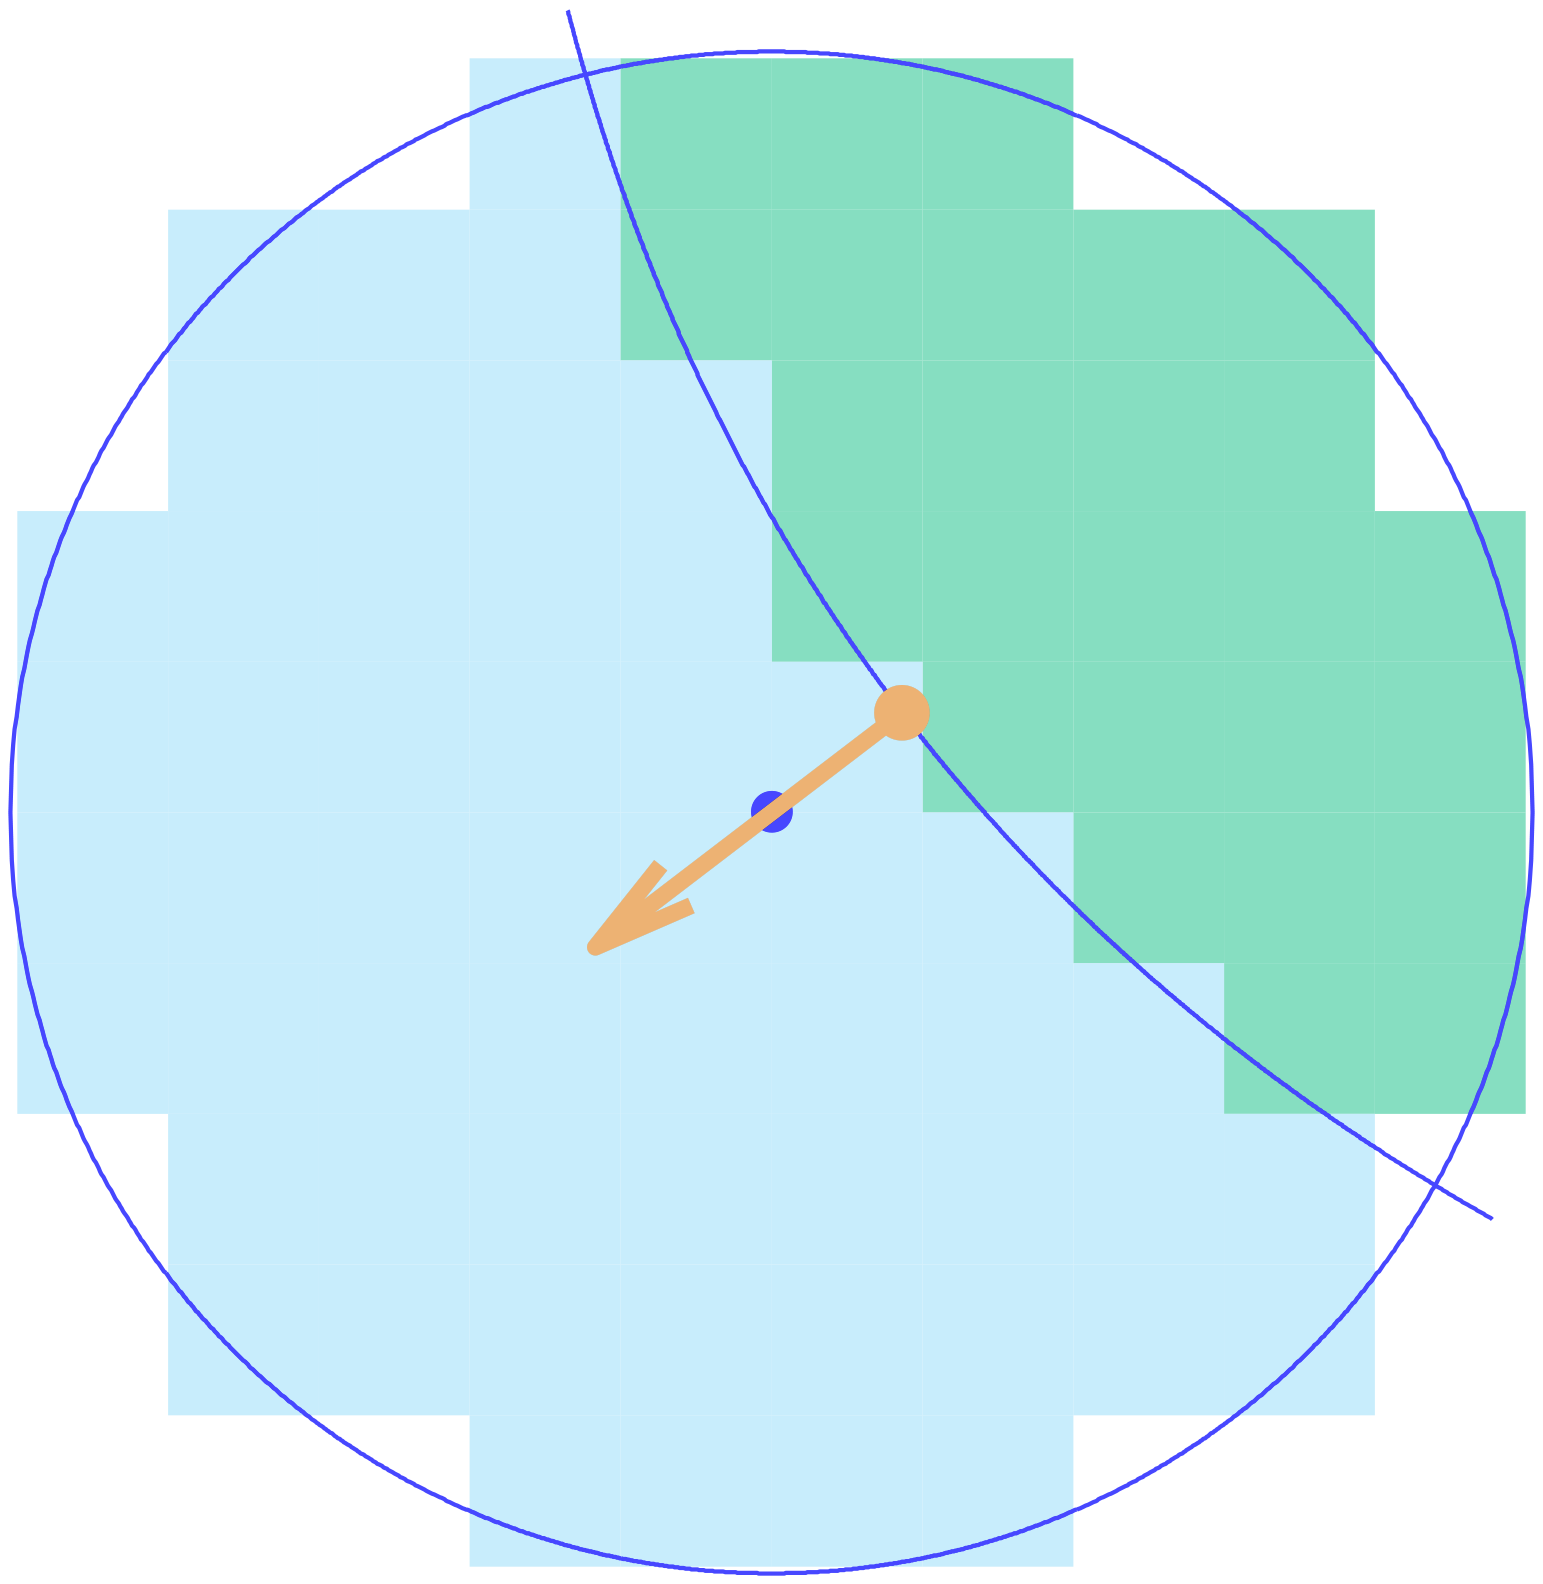
\includegraphics[scale=0.57]{media/2-shabaka/1-vor/dem3.png}
\label{fig:vor3}}
\subfigure[]{%
		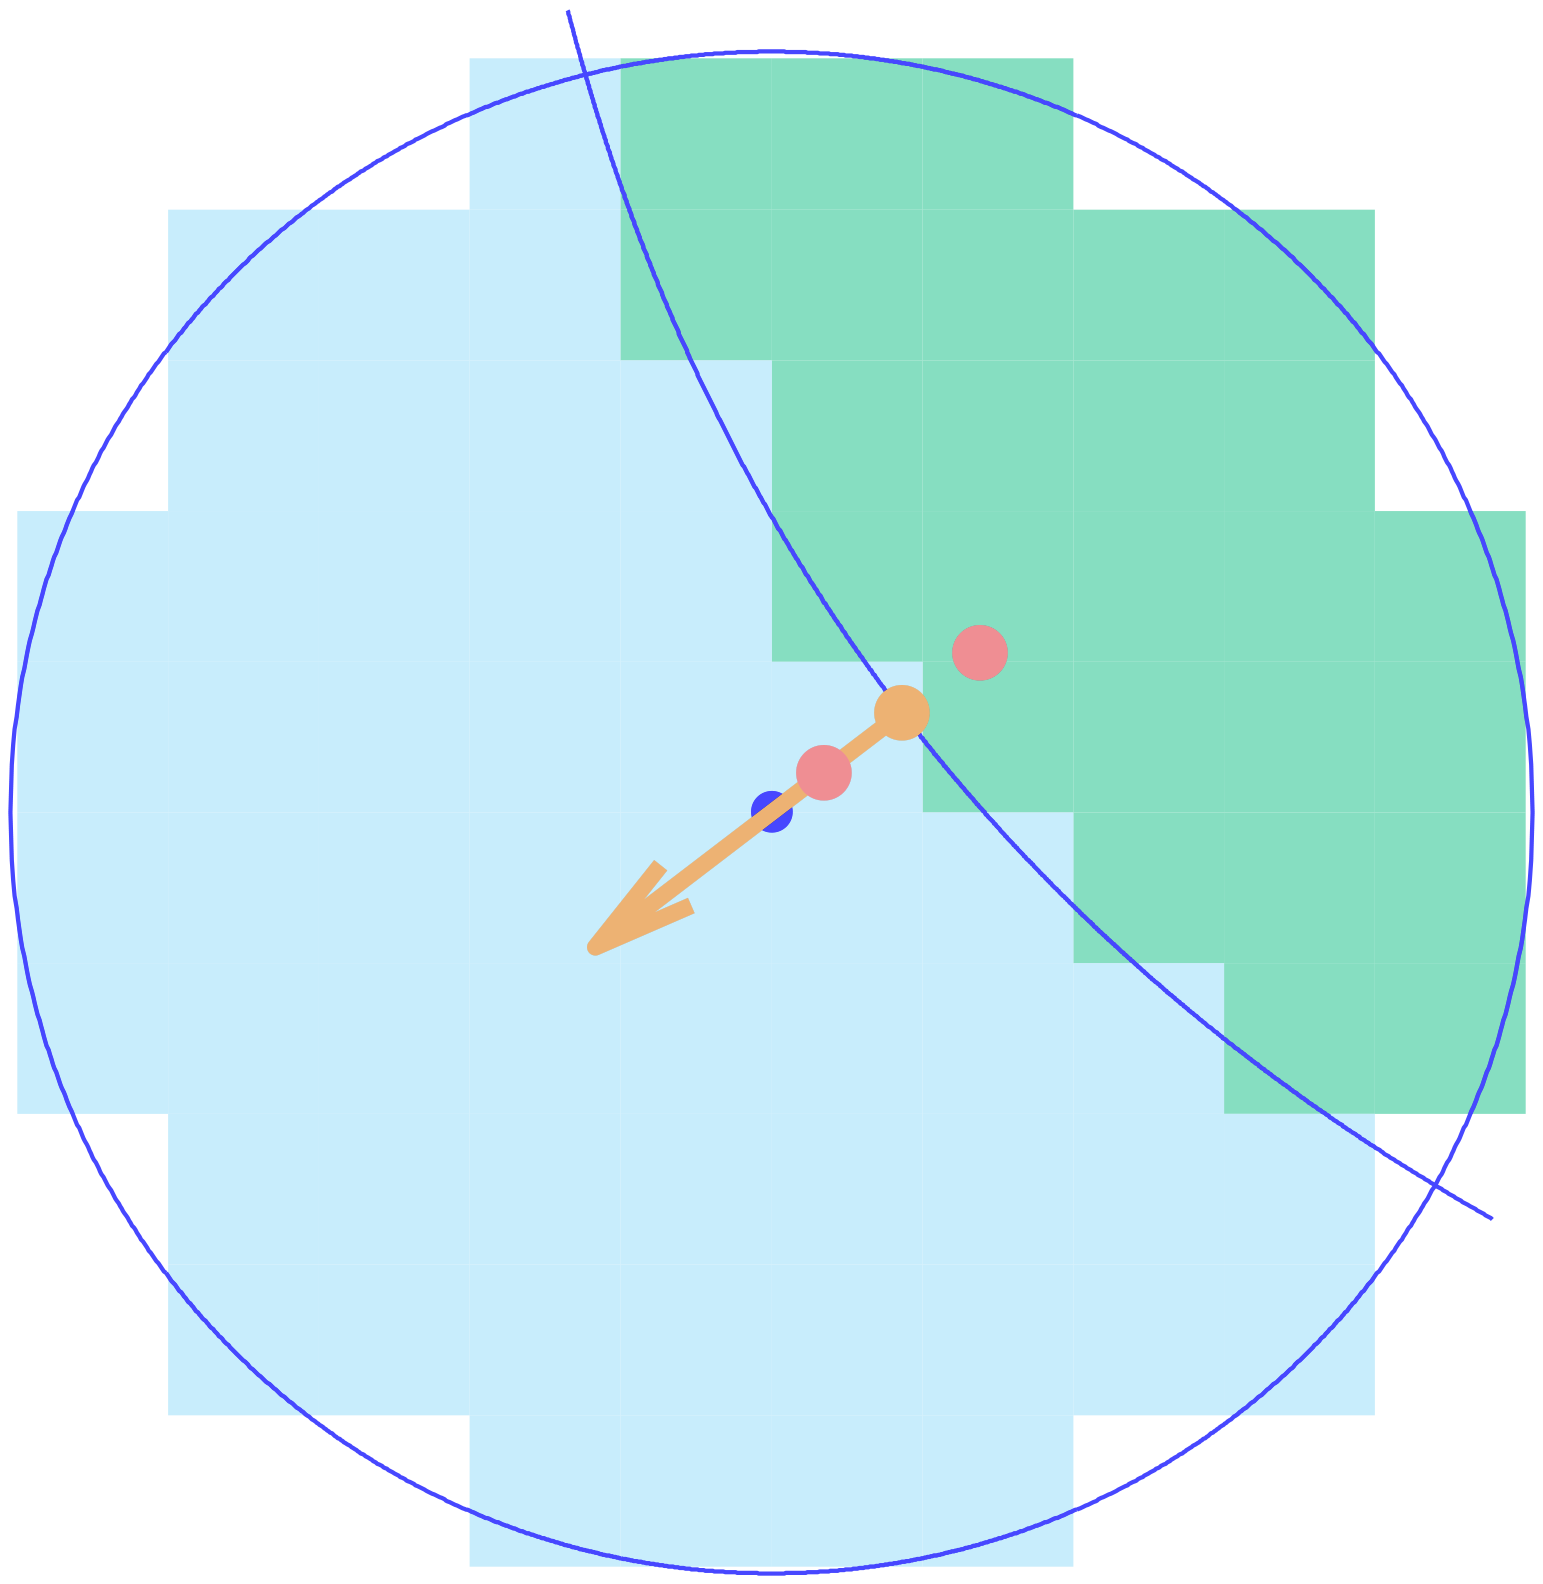
\includegraphics[scale=0.57]{media/2-shabaka/1-vor/dem4.png}
\label{fig:vor4}}
%
\caption{(a) Sample window of segmented image, (b) interface approximation, (c) point/normal placement, and d) Voronoi site placement}
\label{fig:vor}
\end{figure}

\begin{figure}[ht]
\centering
\subfigure[]{%
		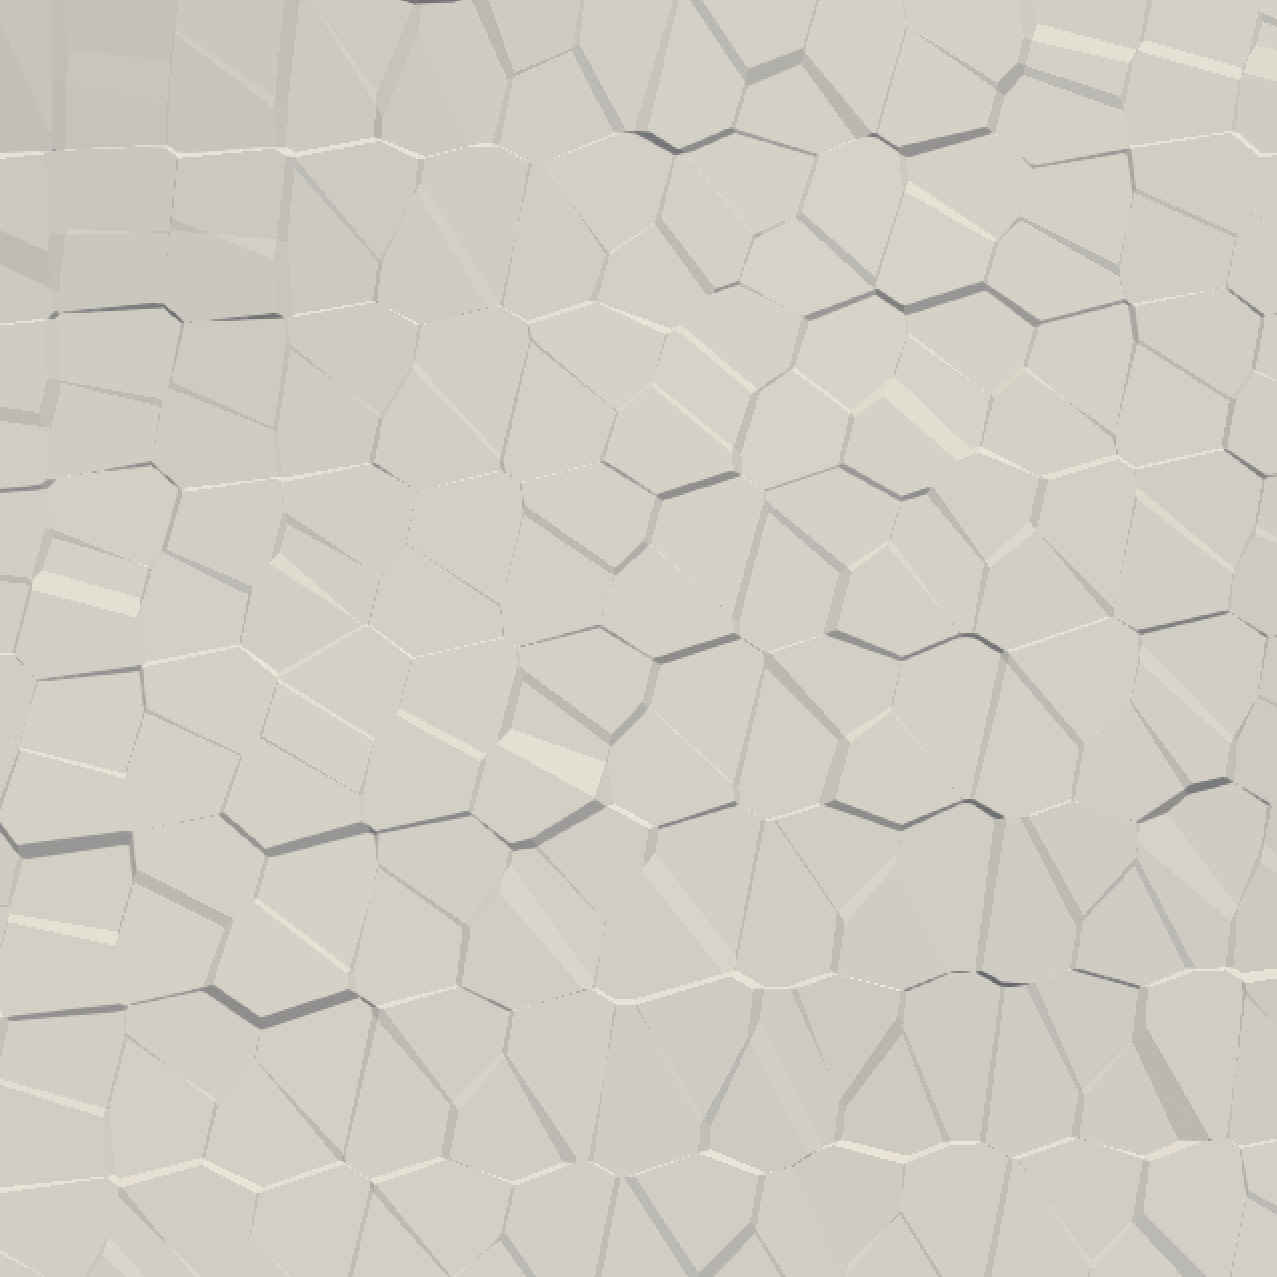
\includegraphics[scale=0.083]{media/2-shabaka/3-clean-zoom/1-init-zoom.png}
\label{fig:cross1-1}}		
\subfigure[]{%
		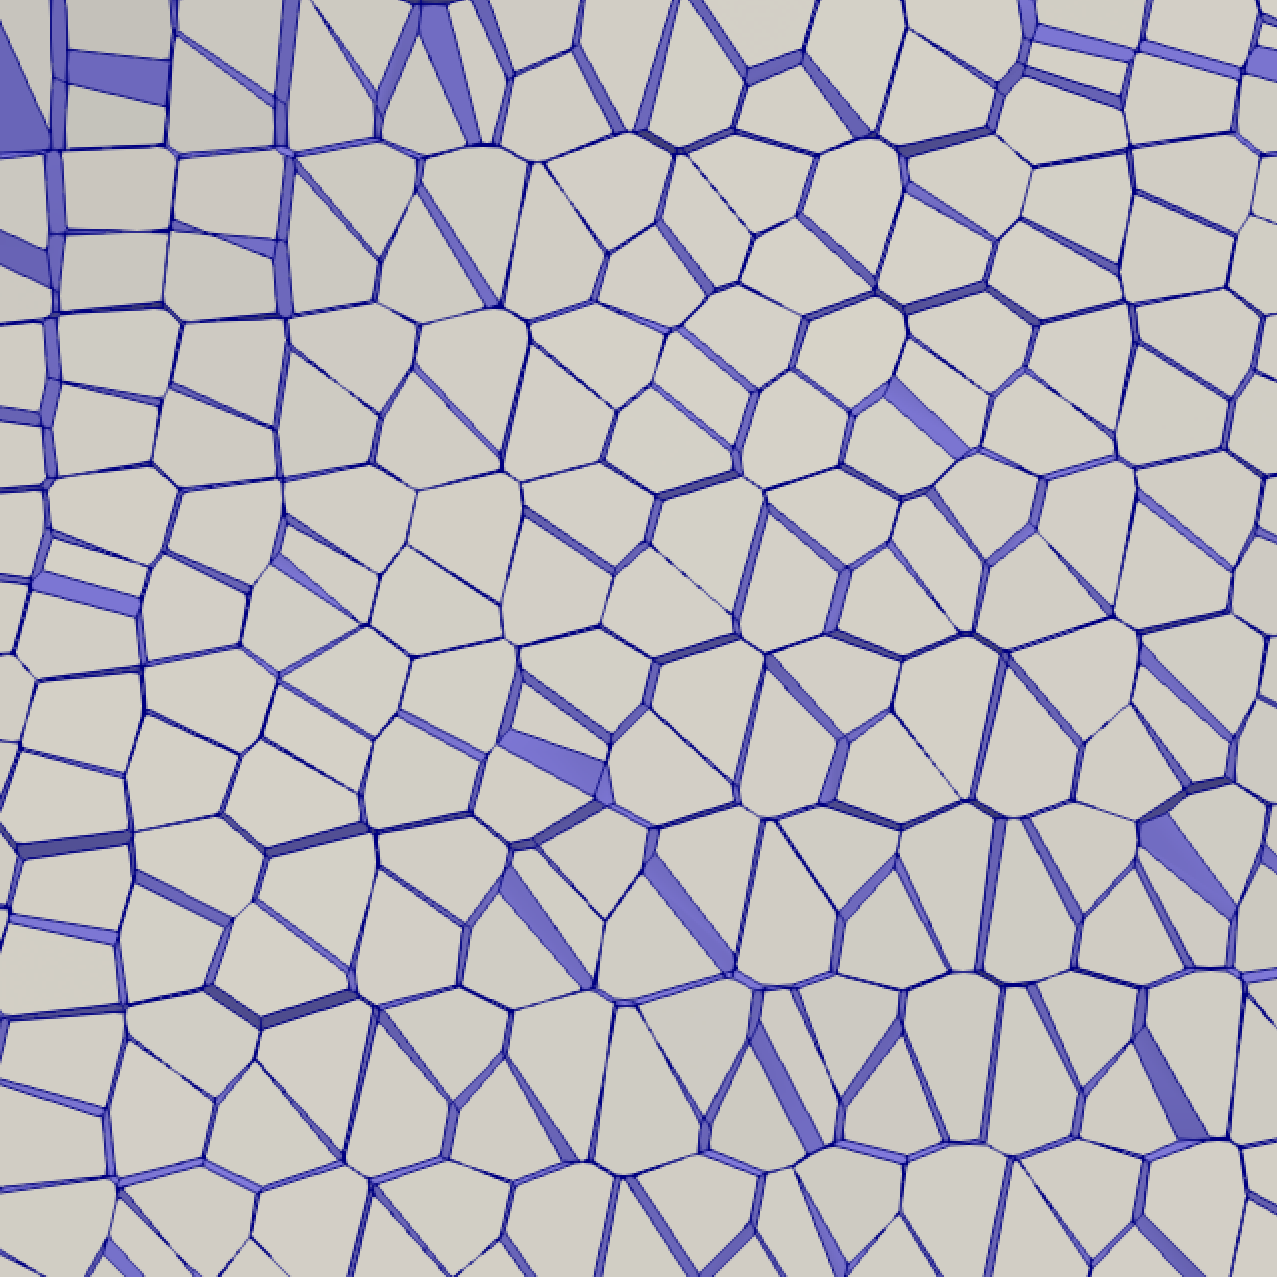
\includegraphics[scale=0.083]{media/2-shabaka/3-clean-zoom/2-badfacets-zoom.png}
\label{fig:cross1-2}}		
\subfigure[]{%
		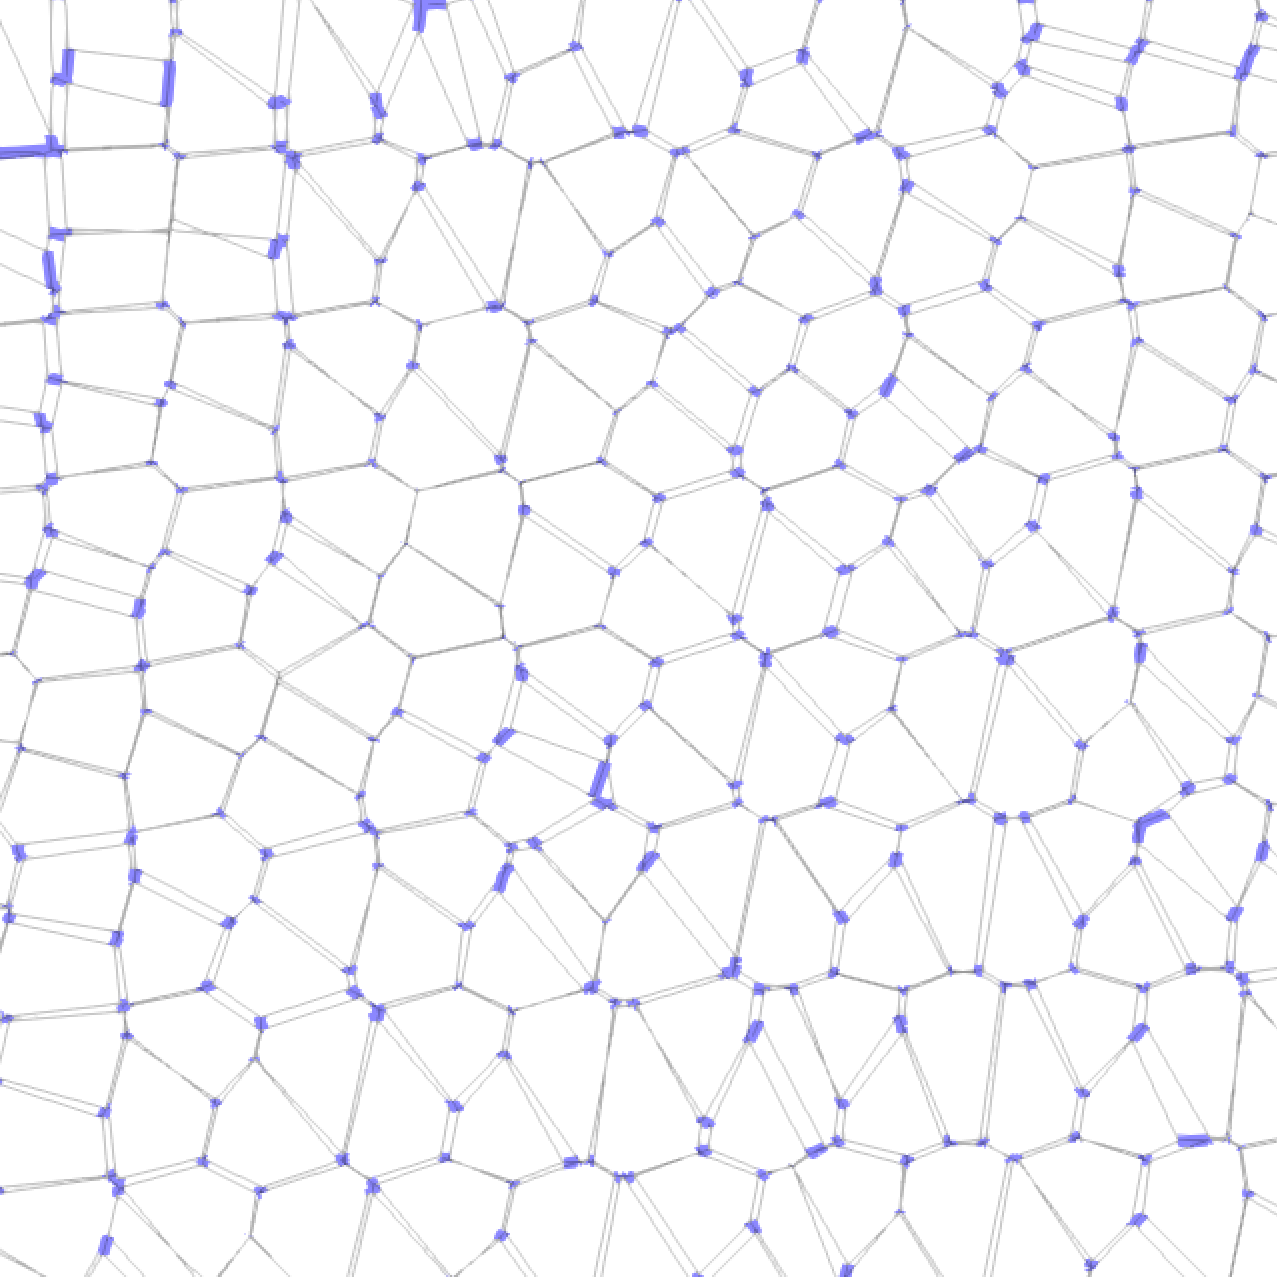
\includegraphics[scale=0.083]{media/2-shabaka/3-clean-zoom/3-badsegs-zoom.png}		
\label{fig:cross1-3}}					
\subfigure[]{%
		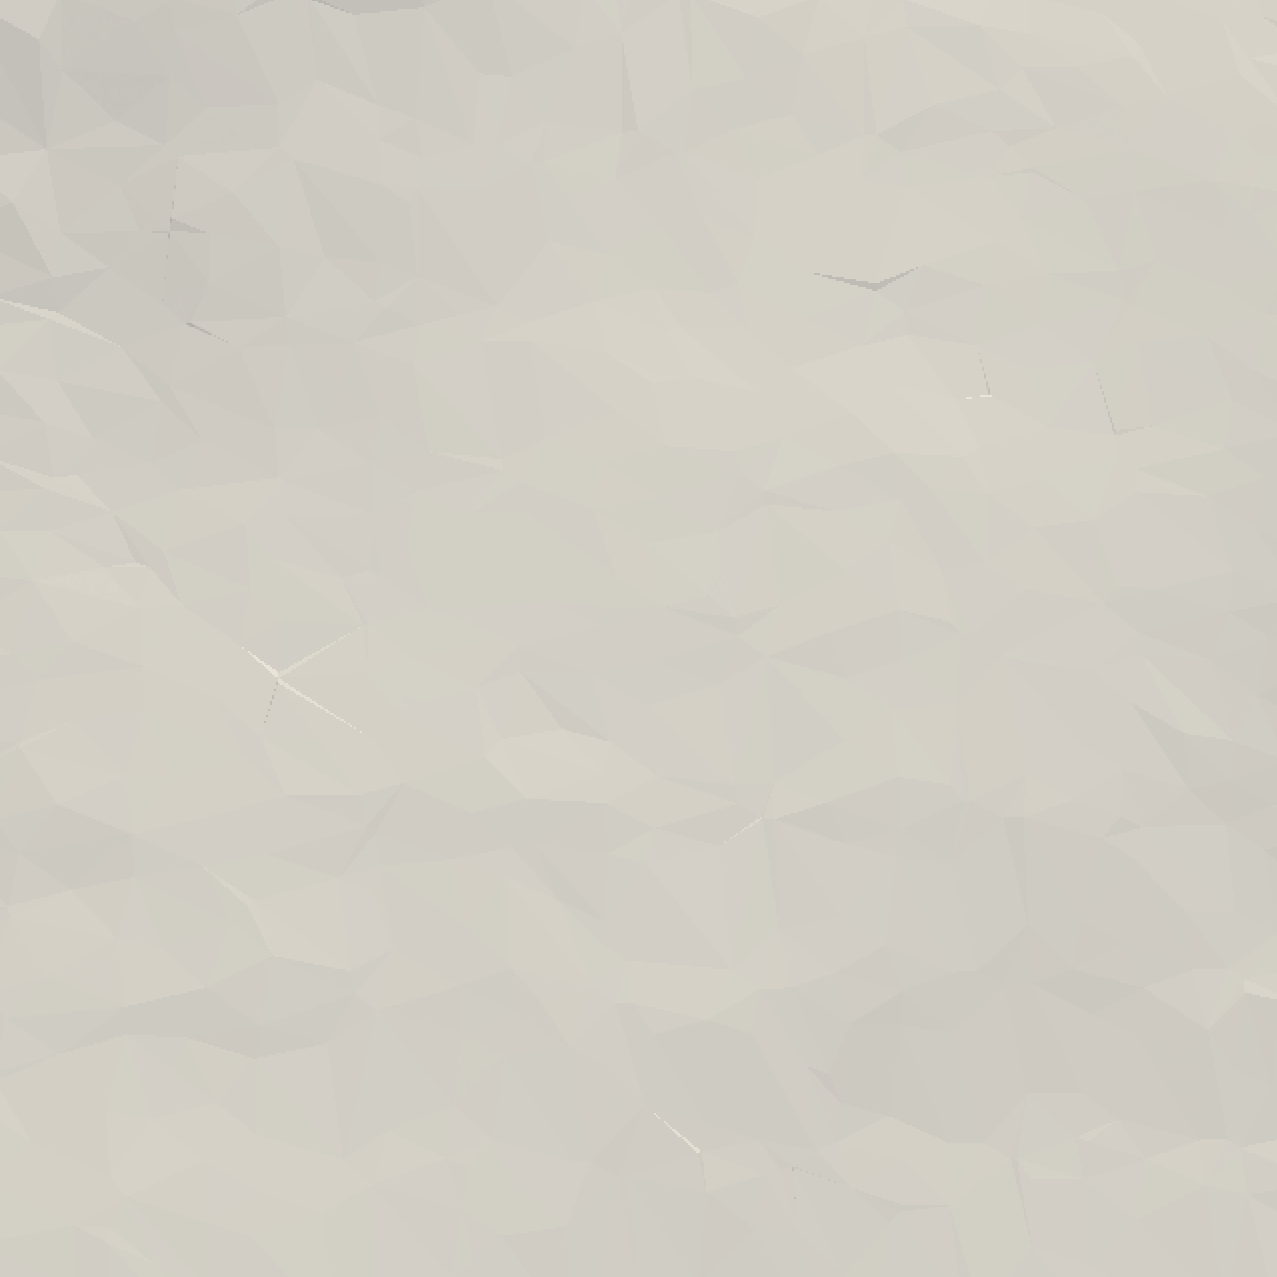
\includegraphics[scale=0.083]{media/2-shabaka/3-clean-zoom/4-fine-zoom.png}
\label{fig:cross1-4}}				
%
\caption{Clean-up of undesirable ``cross-talk'' facets for a surface patch: (a) initial surface following Voronoi-based surface reconstruction, (b) identification of ``cross-talk'' facets, (c) identification of edges to be collapsed, (d) final cleaned surface.}
\label{fig:cross1}
\end{figure}

\begin{figure}[ht]
\centering
\subfigure[]{%
		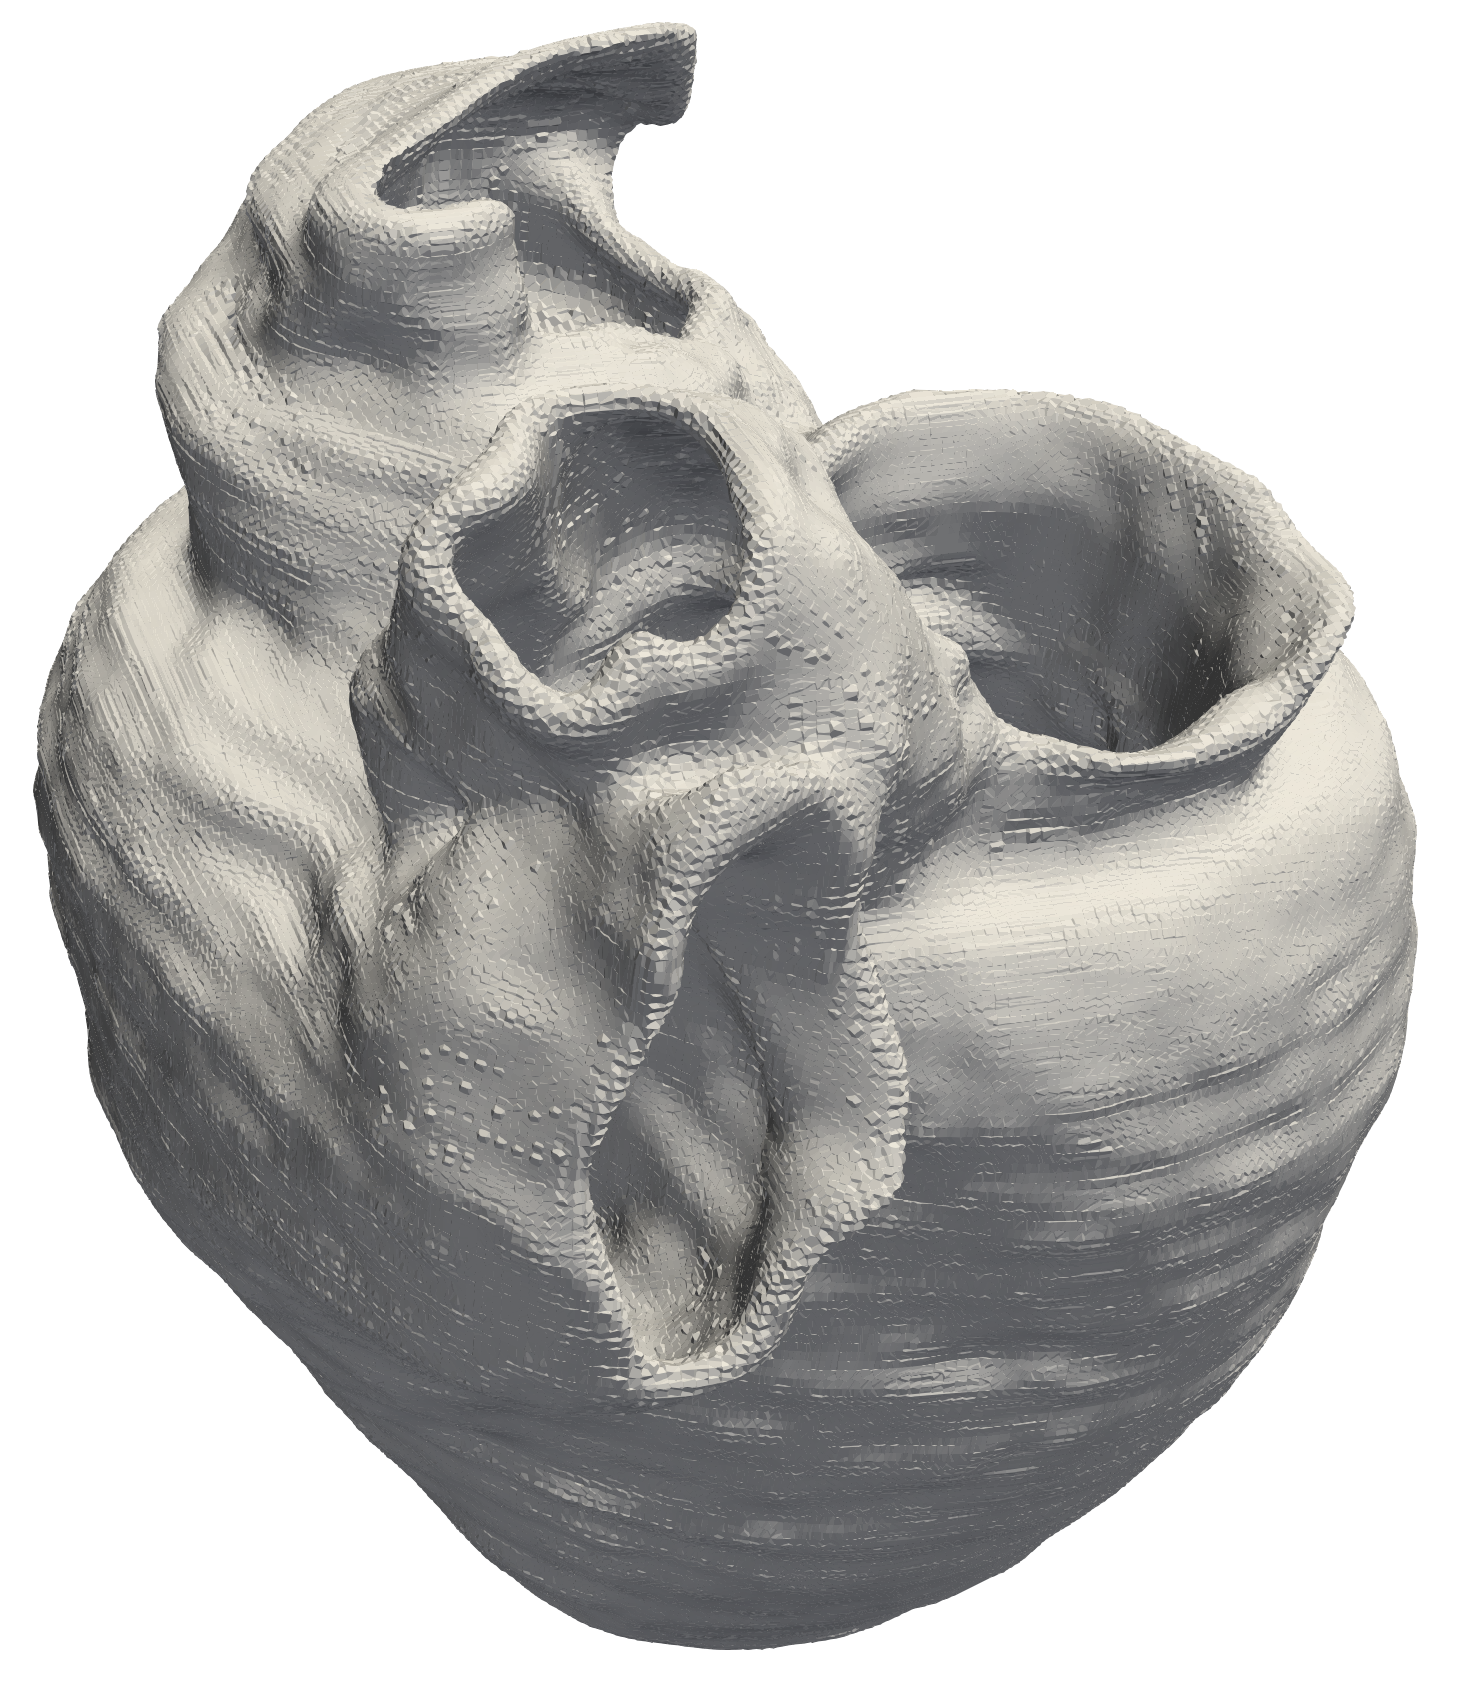
\includegraphics[scale=0.07]{media/2-shabaka/4-clean/1-init.png}
\label{fig:cross2-1}}		
\subfigure[]{%
		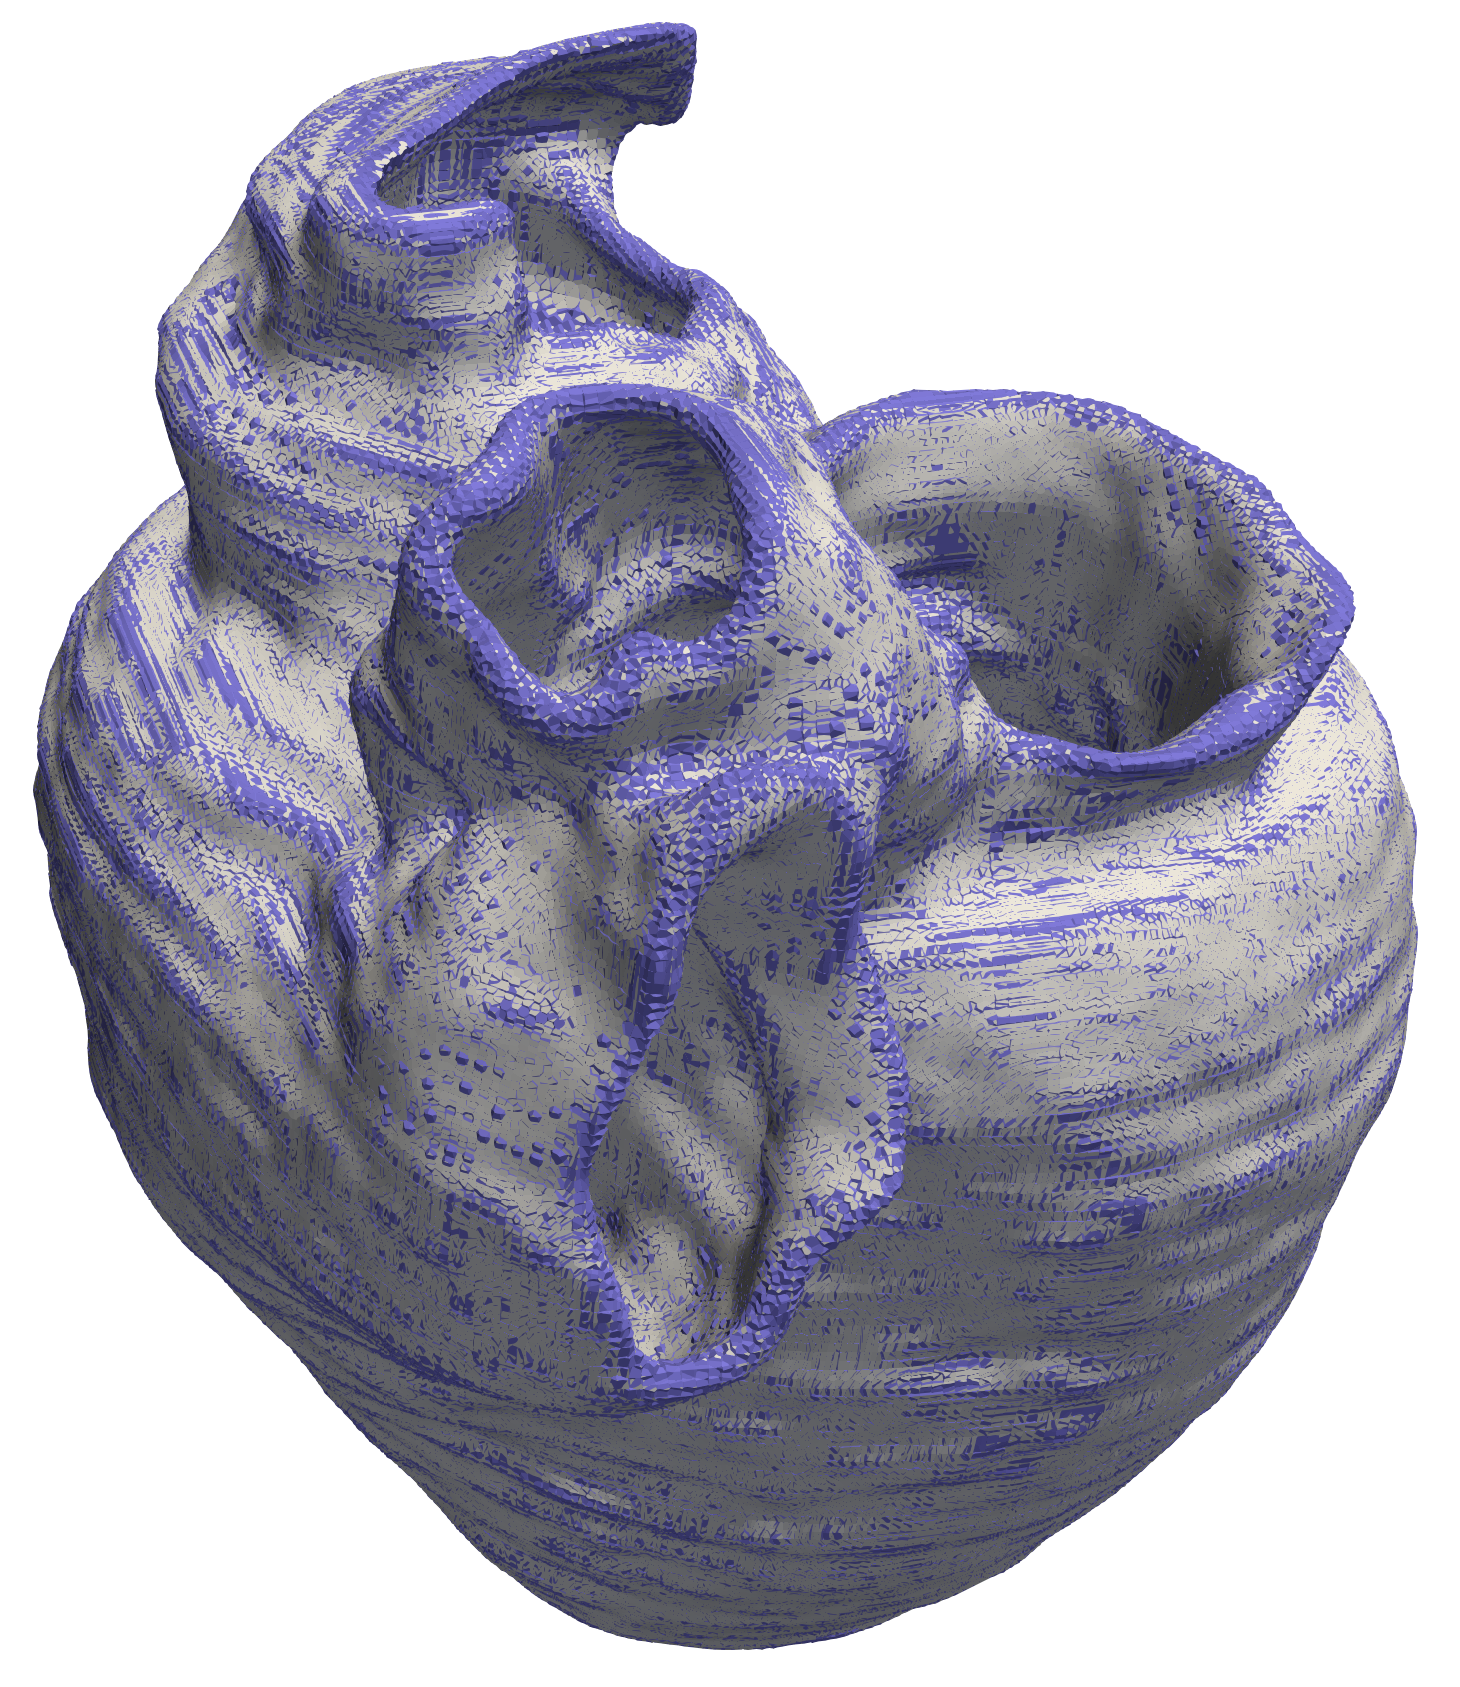
\includegraphics[scale=0.07]{media/2-shabaka/4-clean/2-badfacets.png}
\label{fig:cross2-2}}		
\subfigure[]{%
		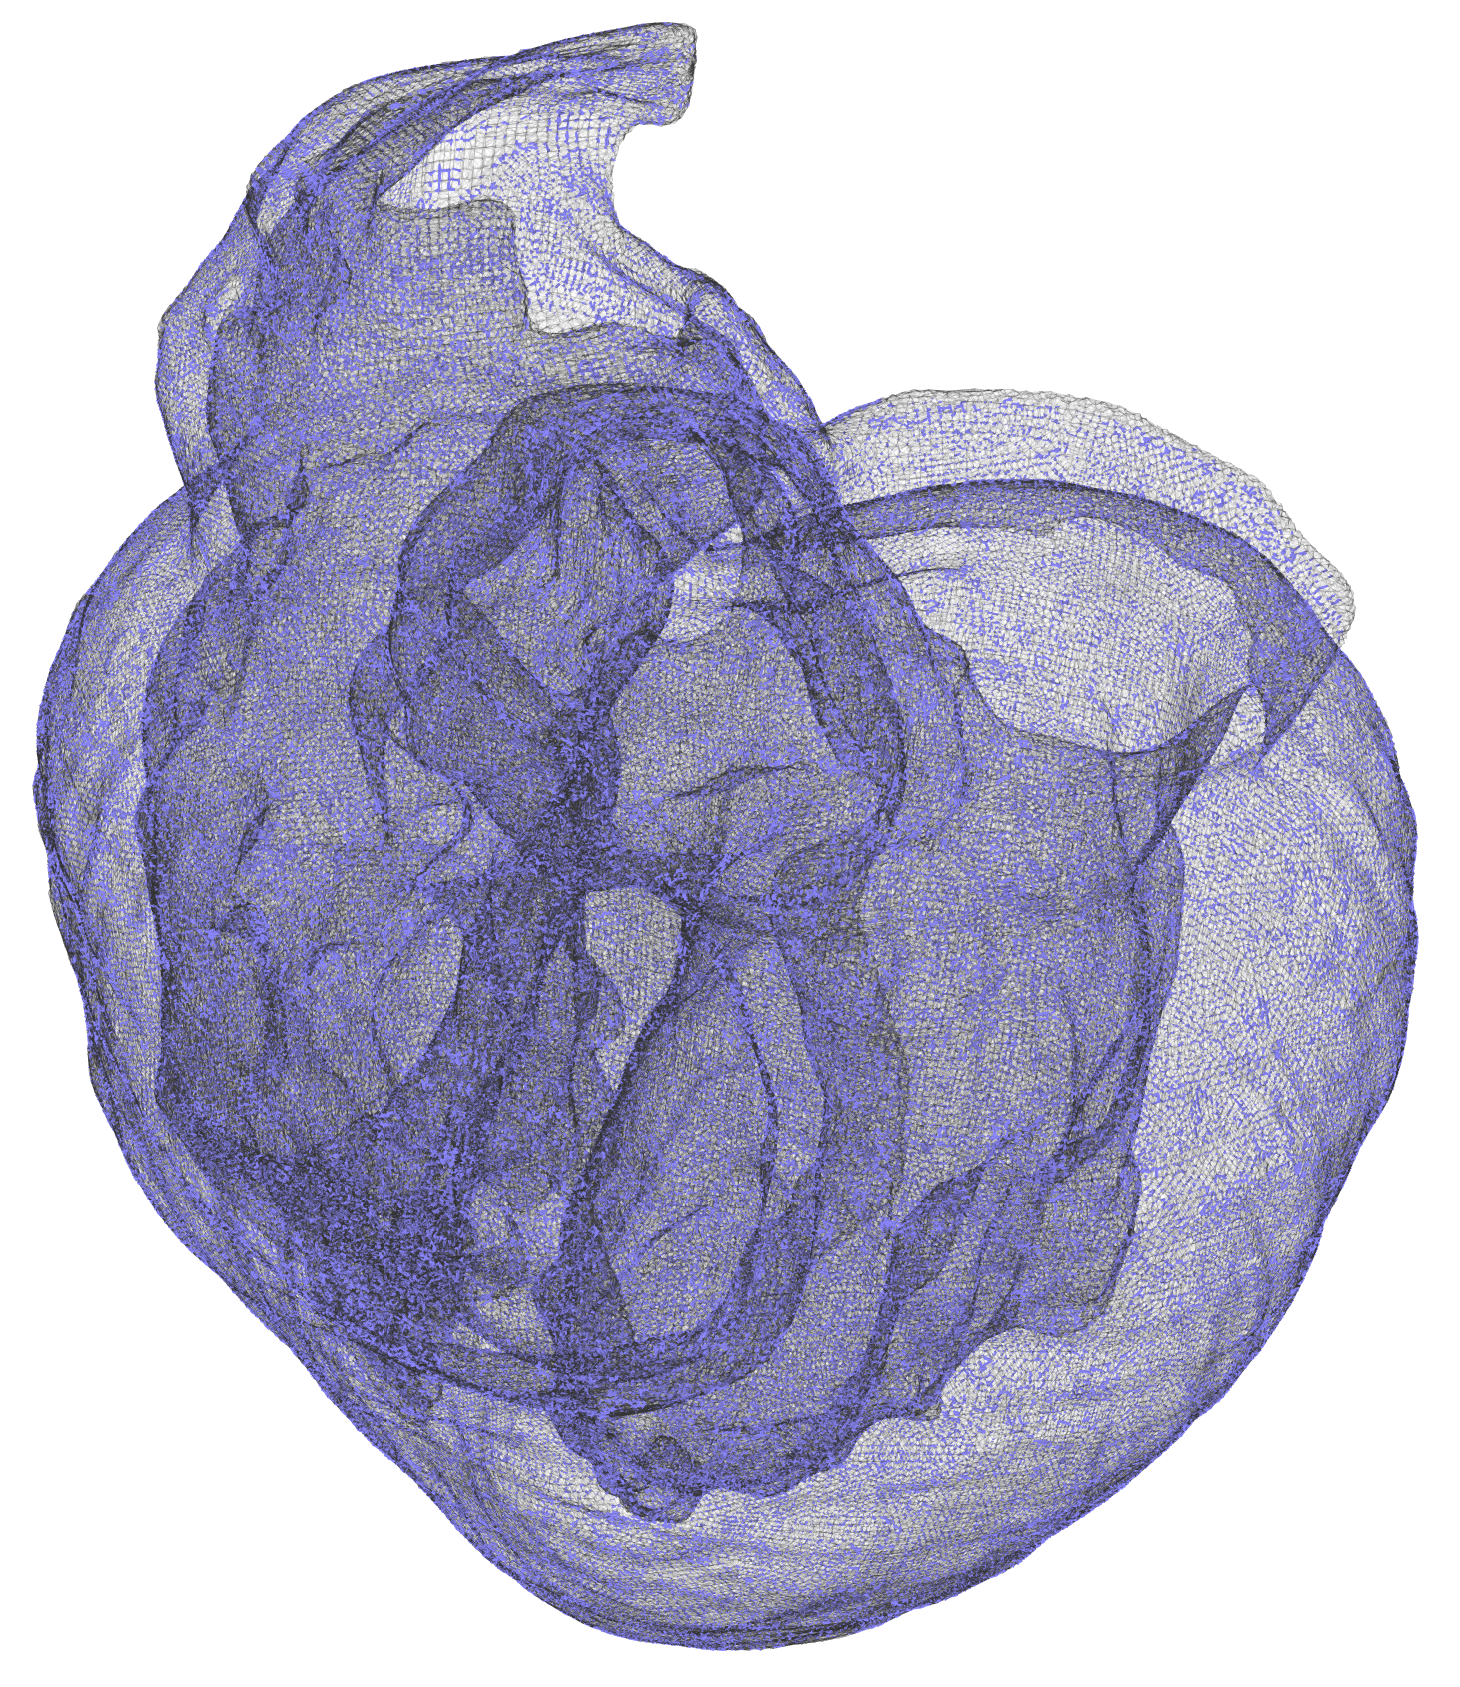
\includegraphics[scale=0.07]{media/2-shabaka/4-clean/3-badsegs.png}	
\label{fig:cross2-3}}						
\subfigure[]{%
		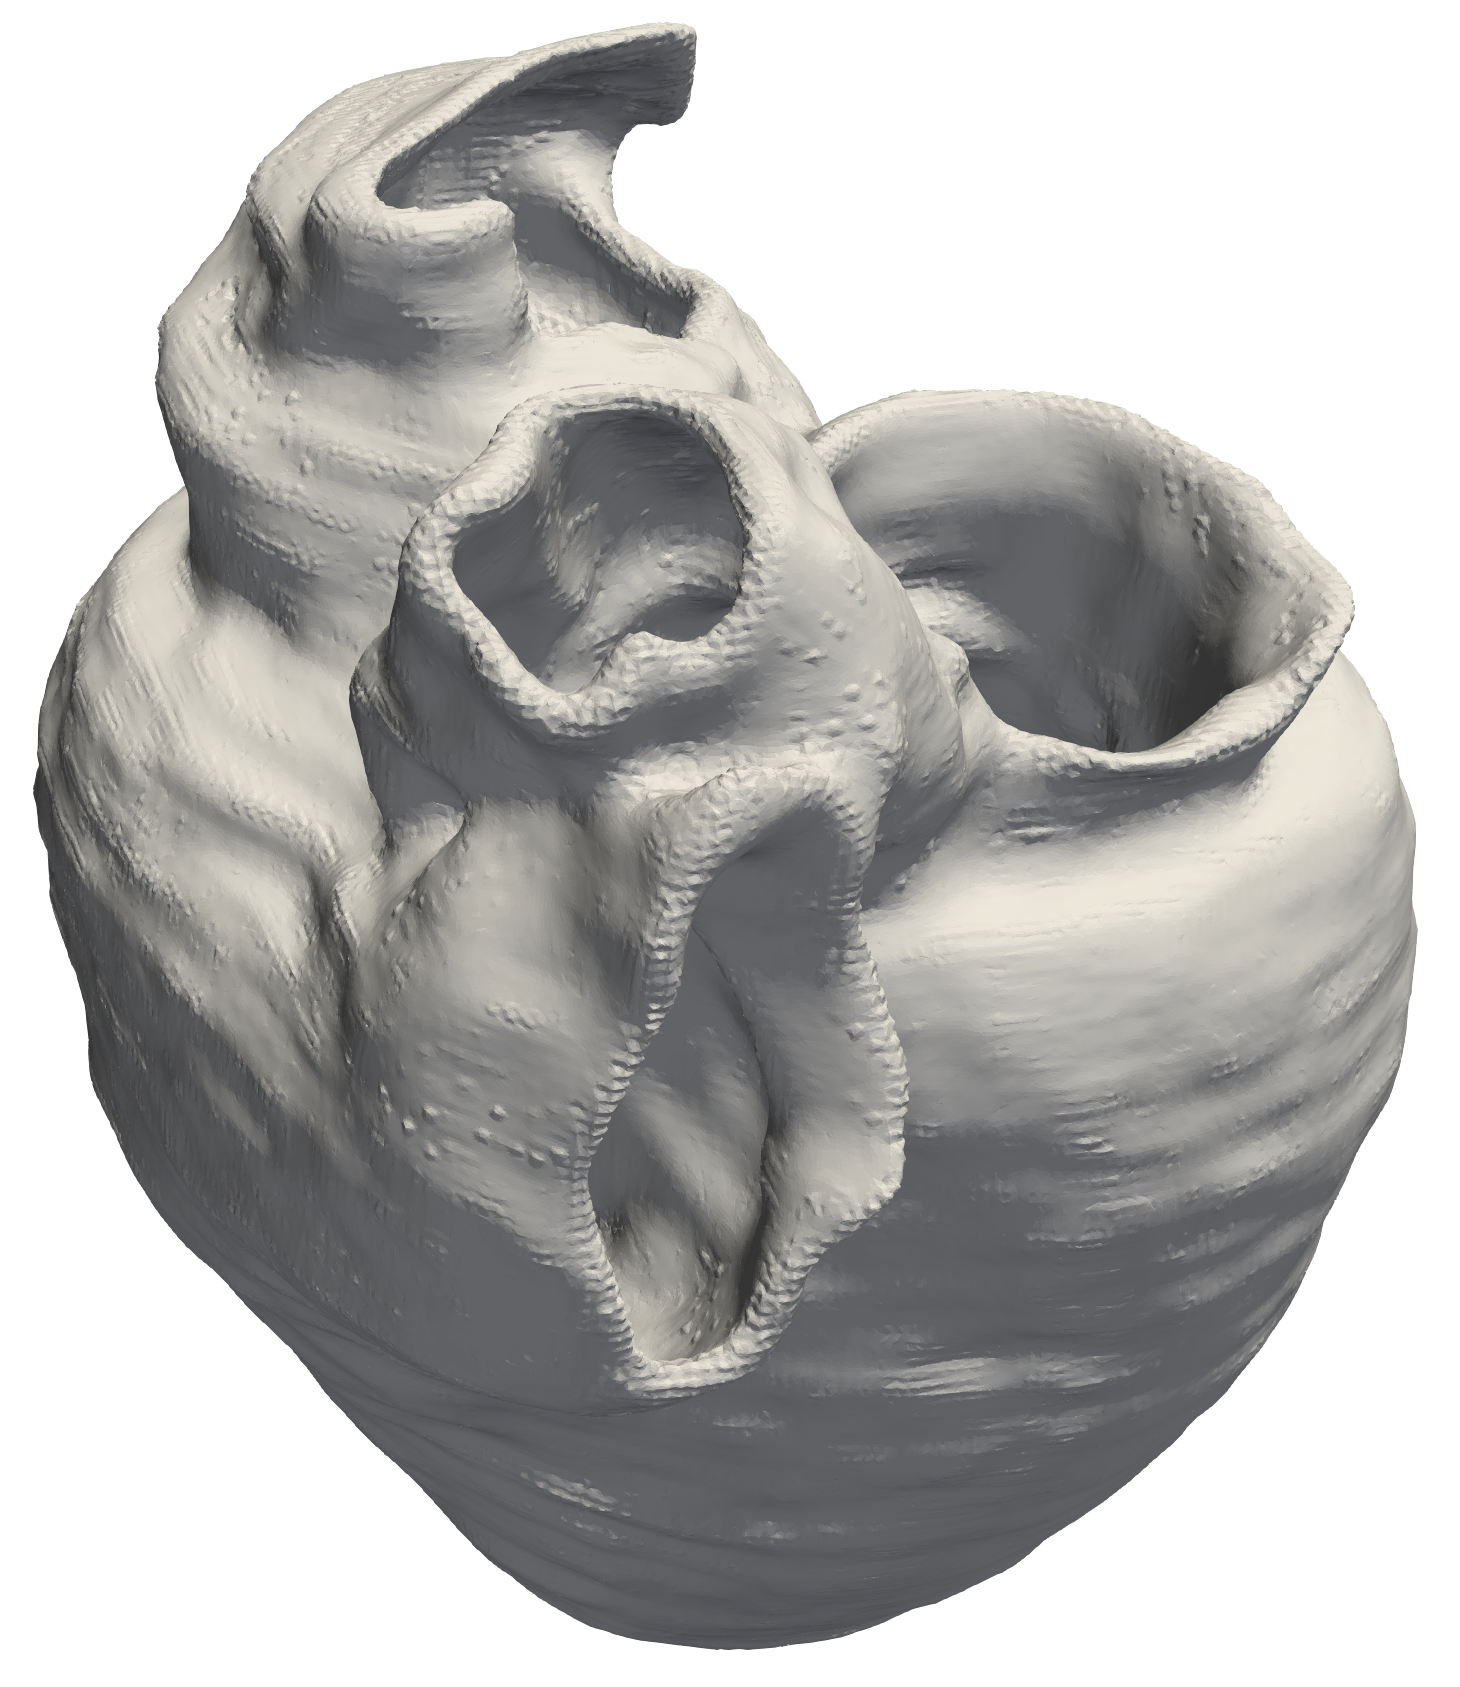
\includegraphics[scale=0.07]{media/2-shabaka/4-clean/4-fine.png}		
\label{fig:cross2-4}}		
%
\caption{Clean-up of undesirable ``cross-talk'' facets for surface of \textit{ex-vivo} human heart: (a) initial surface following Voronoi-based surface reconstruction, (b) identification of ``cross-talk'' facets, (c) identification of edges to be collapsed, (d) final cleaned surface.}
\label{fig:cross2}
\end{figure}

\begin{figure}[ht!]
\centering
\subfigure[]{%
		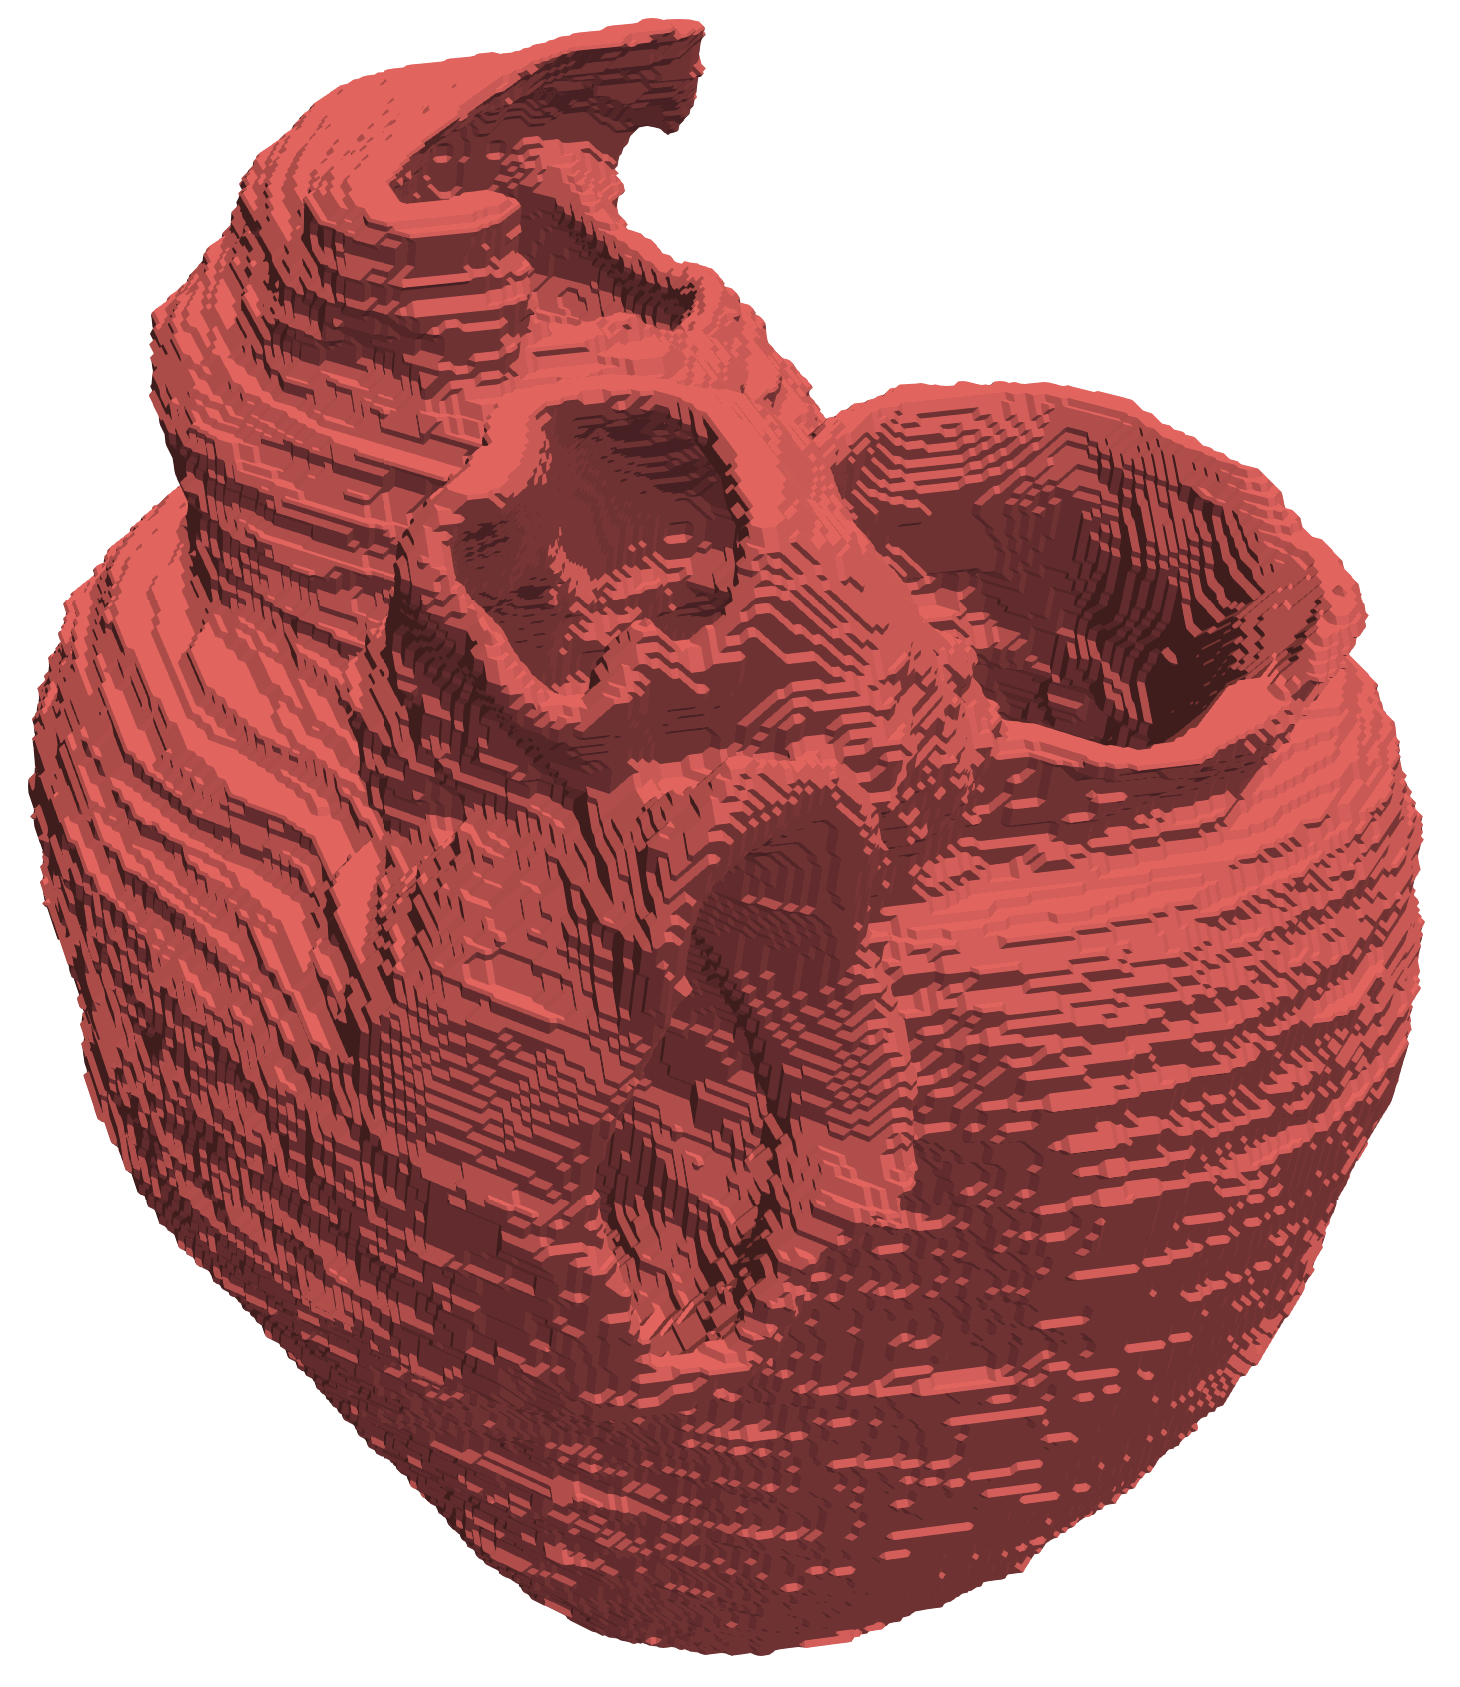
\includegraphics[scale=0.092]{media/2-shabaka/2-surf/1-seg.png}
\label{fig:shabakaseq1}}
\subfigure[]{%
		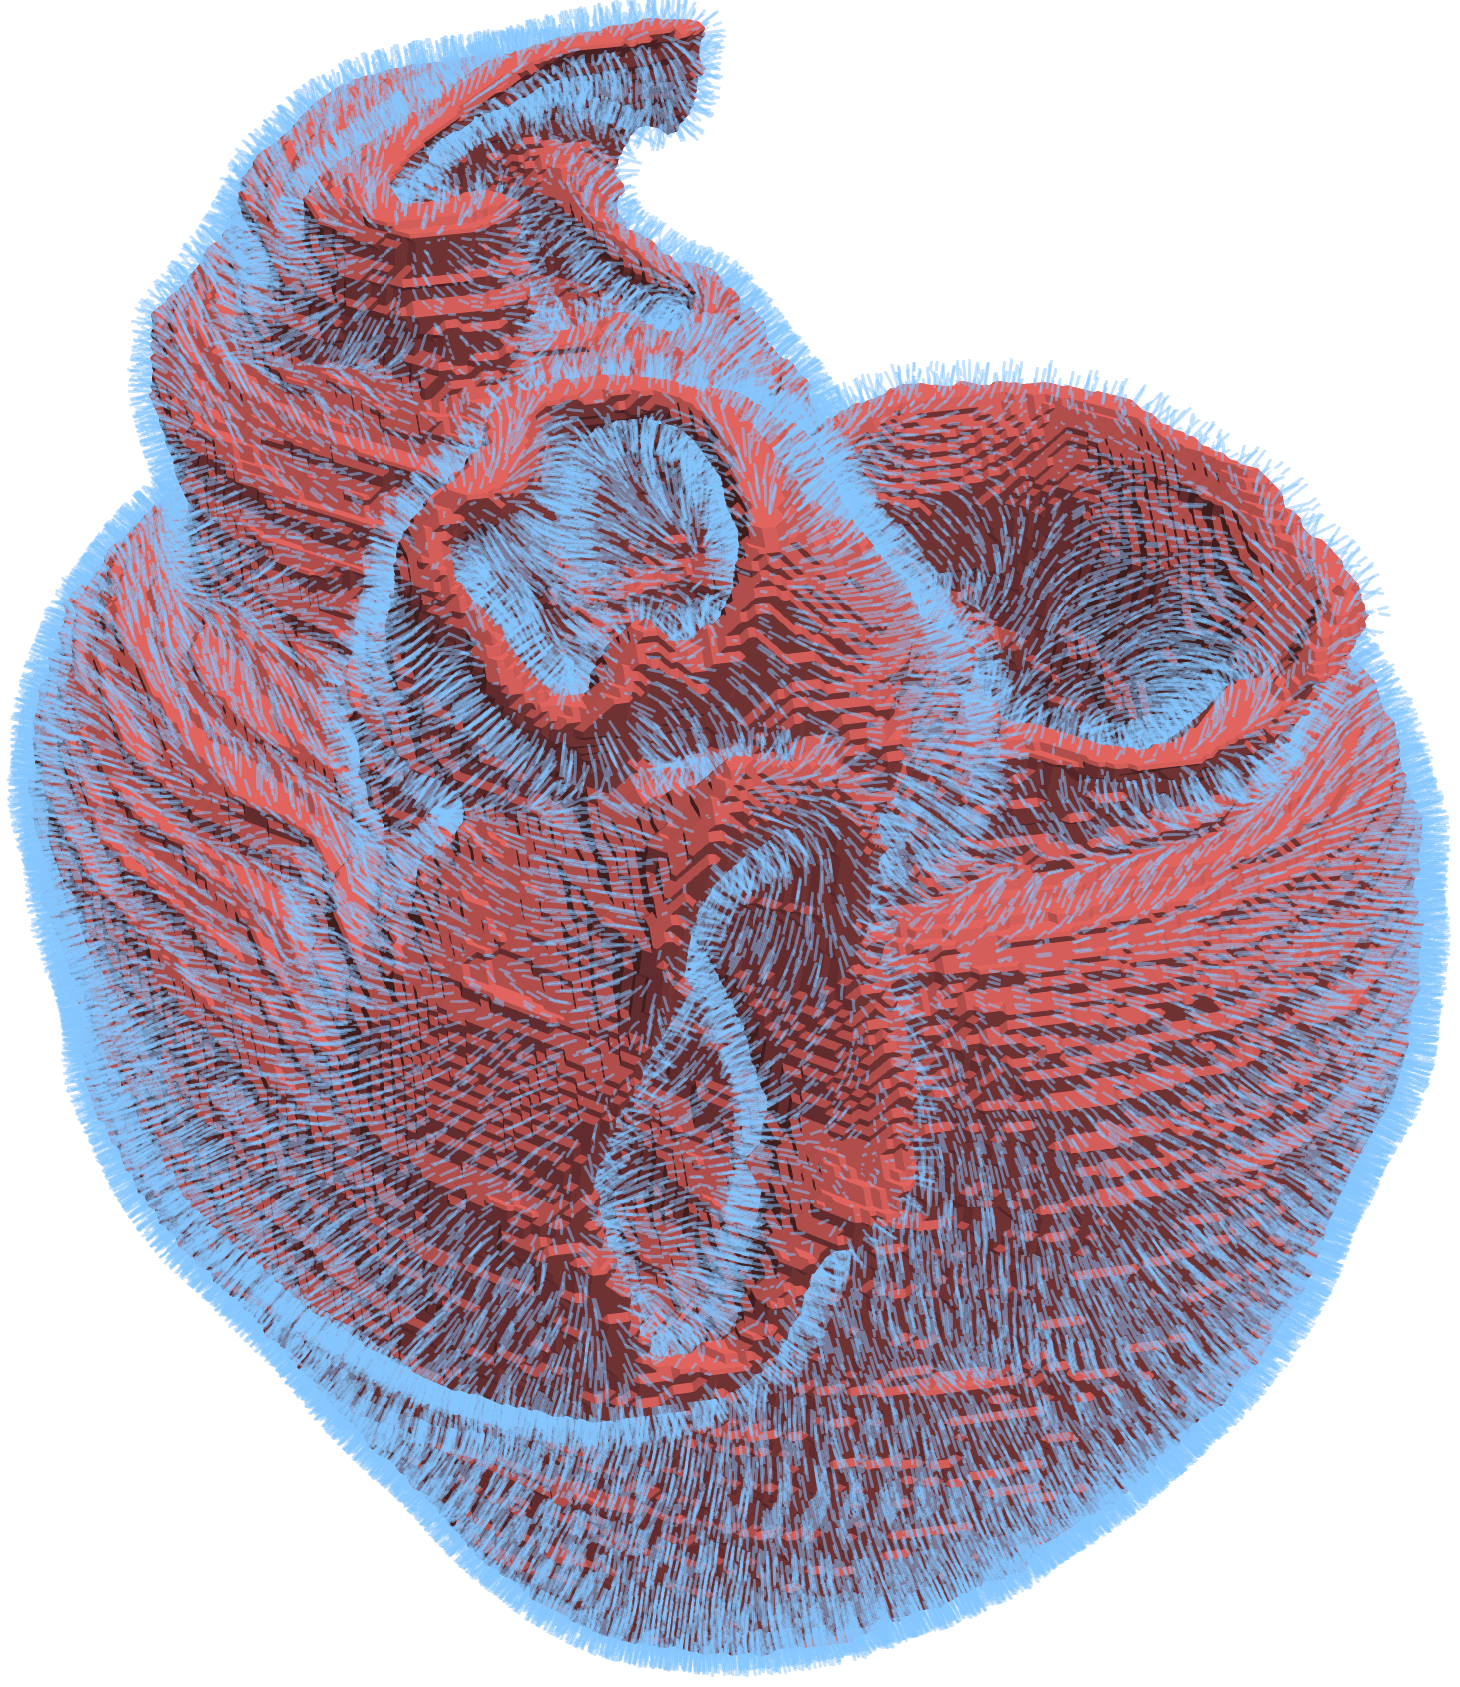
\includegraphics[scale=0.092]{media/2-shabaka/2-surf/2-normals.png}
\label{fig:shabakaseq2}}
\subfigure[]{%
		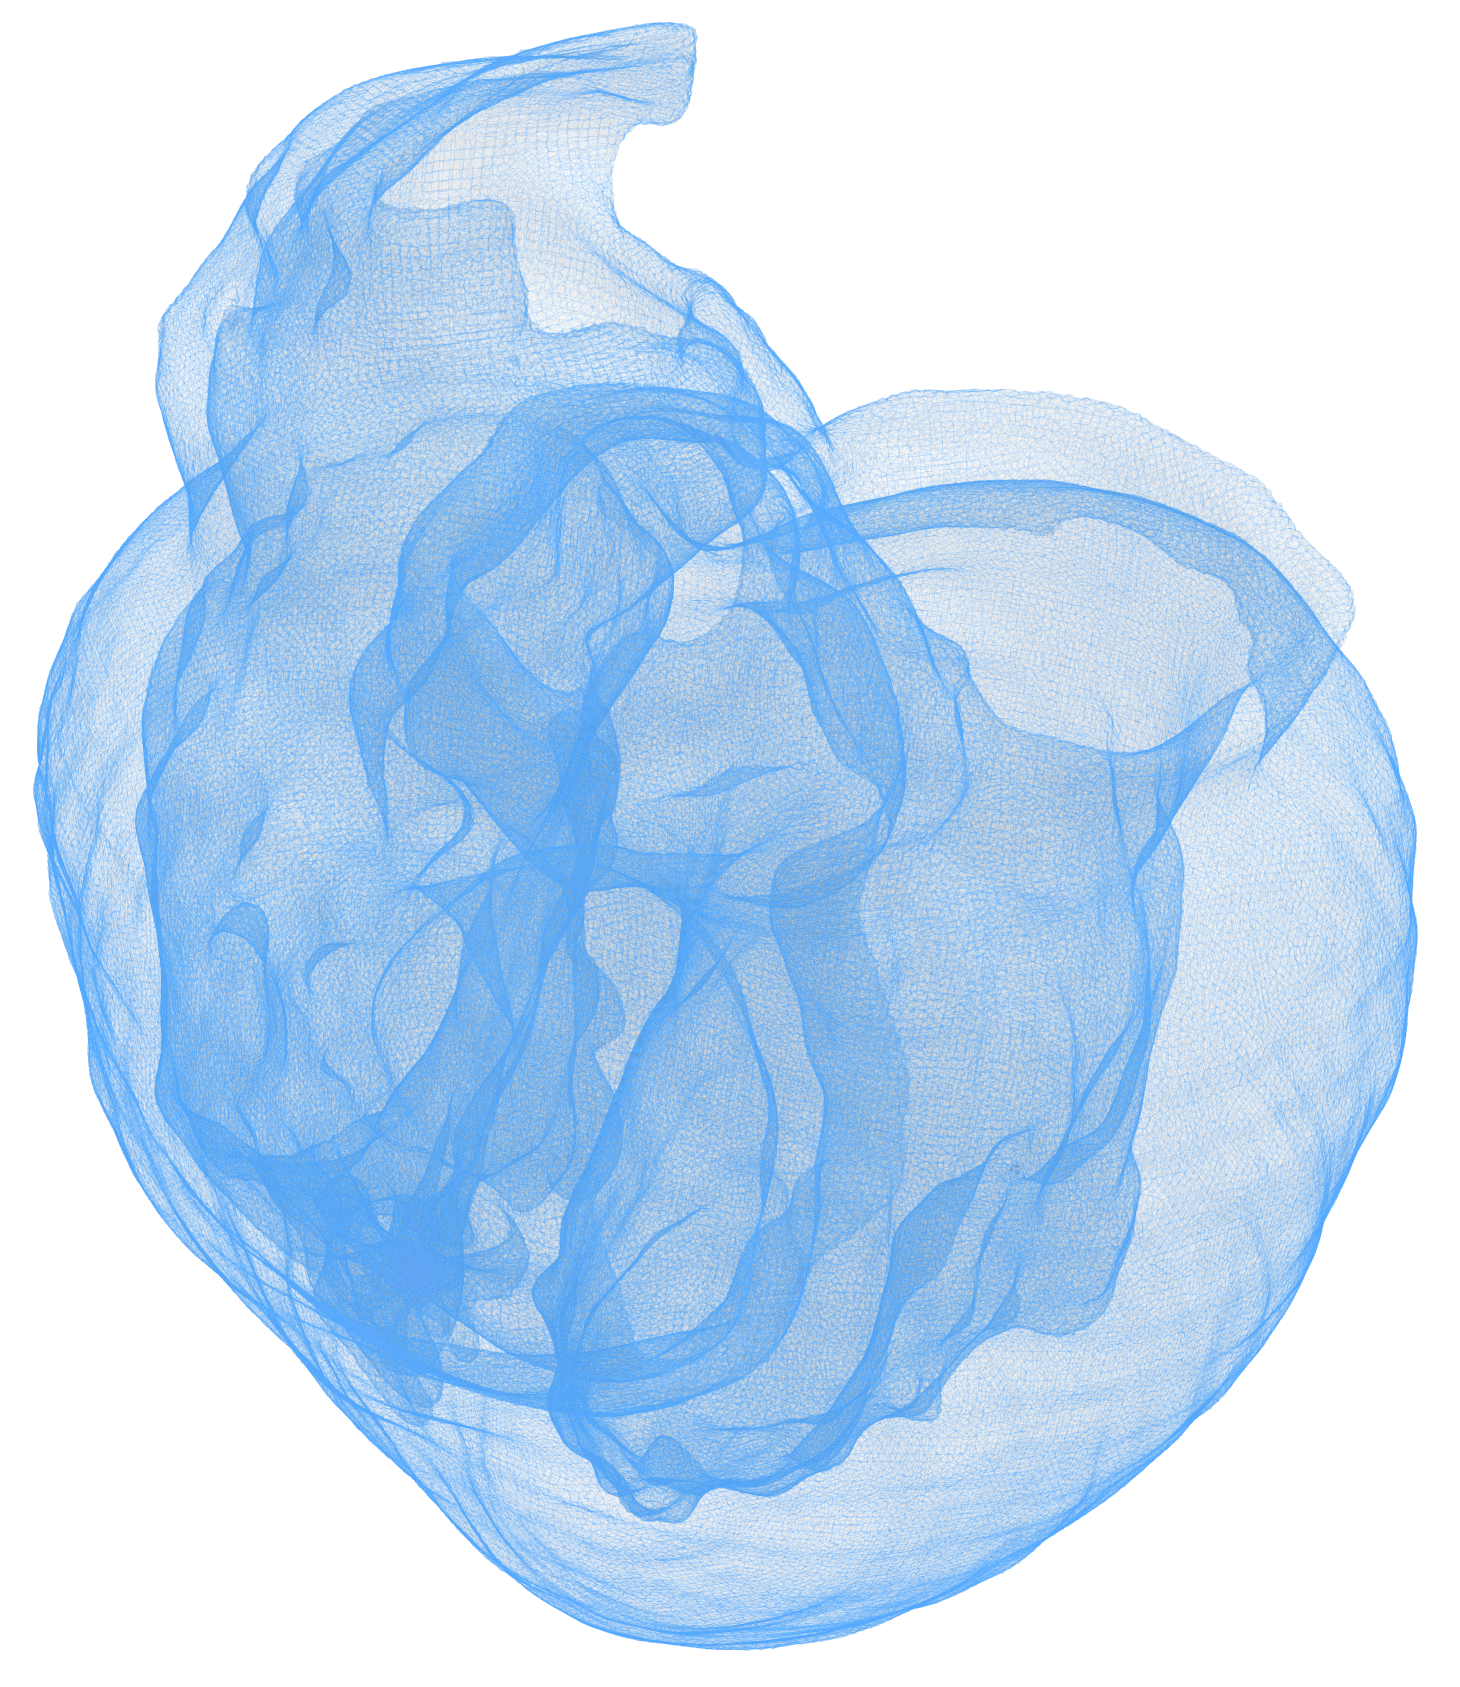
\includegraphics[scale=0.092]{media/2-shabaka/2-surf/3-ptcloud.png}
\label{fig:shabakaseq3}}
\subfigure[]{%
		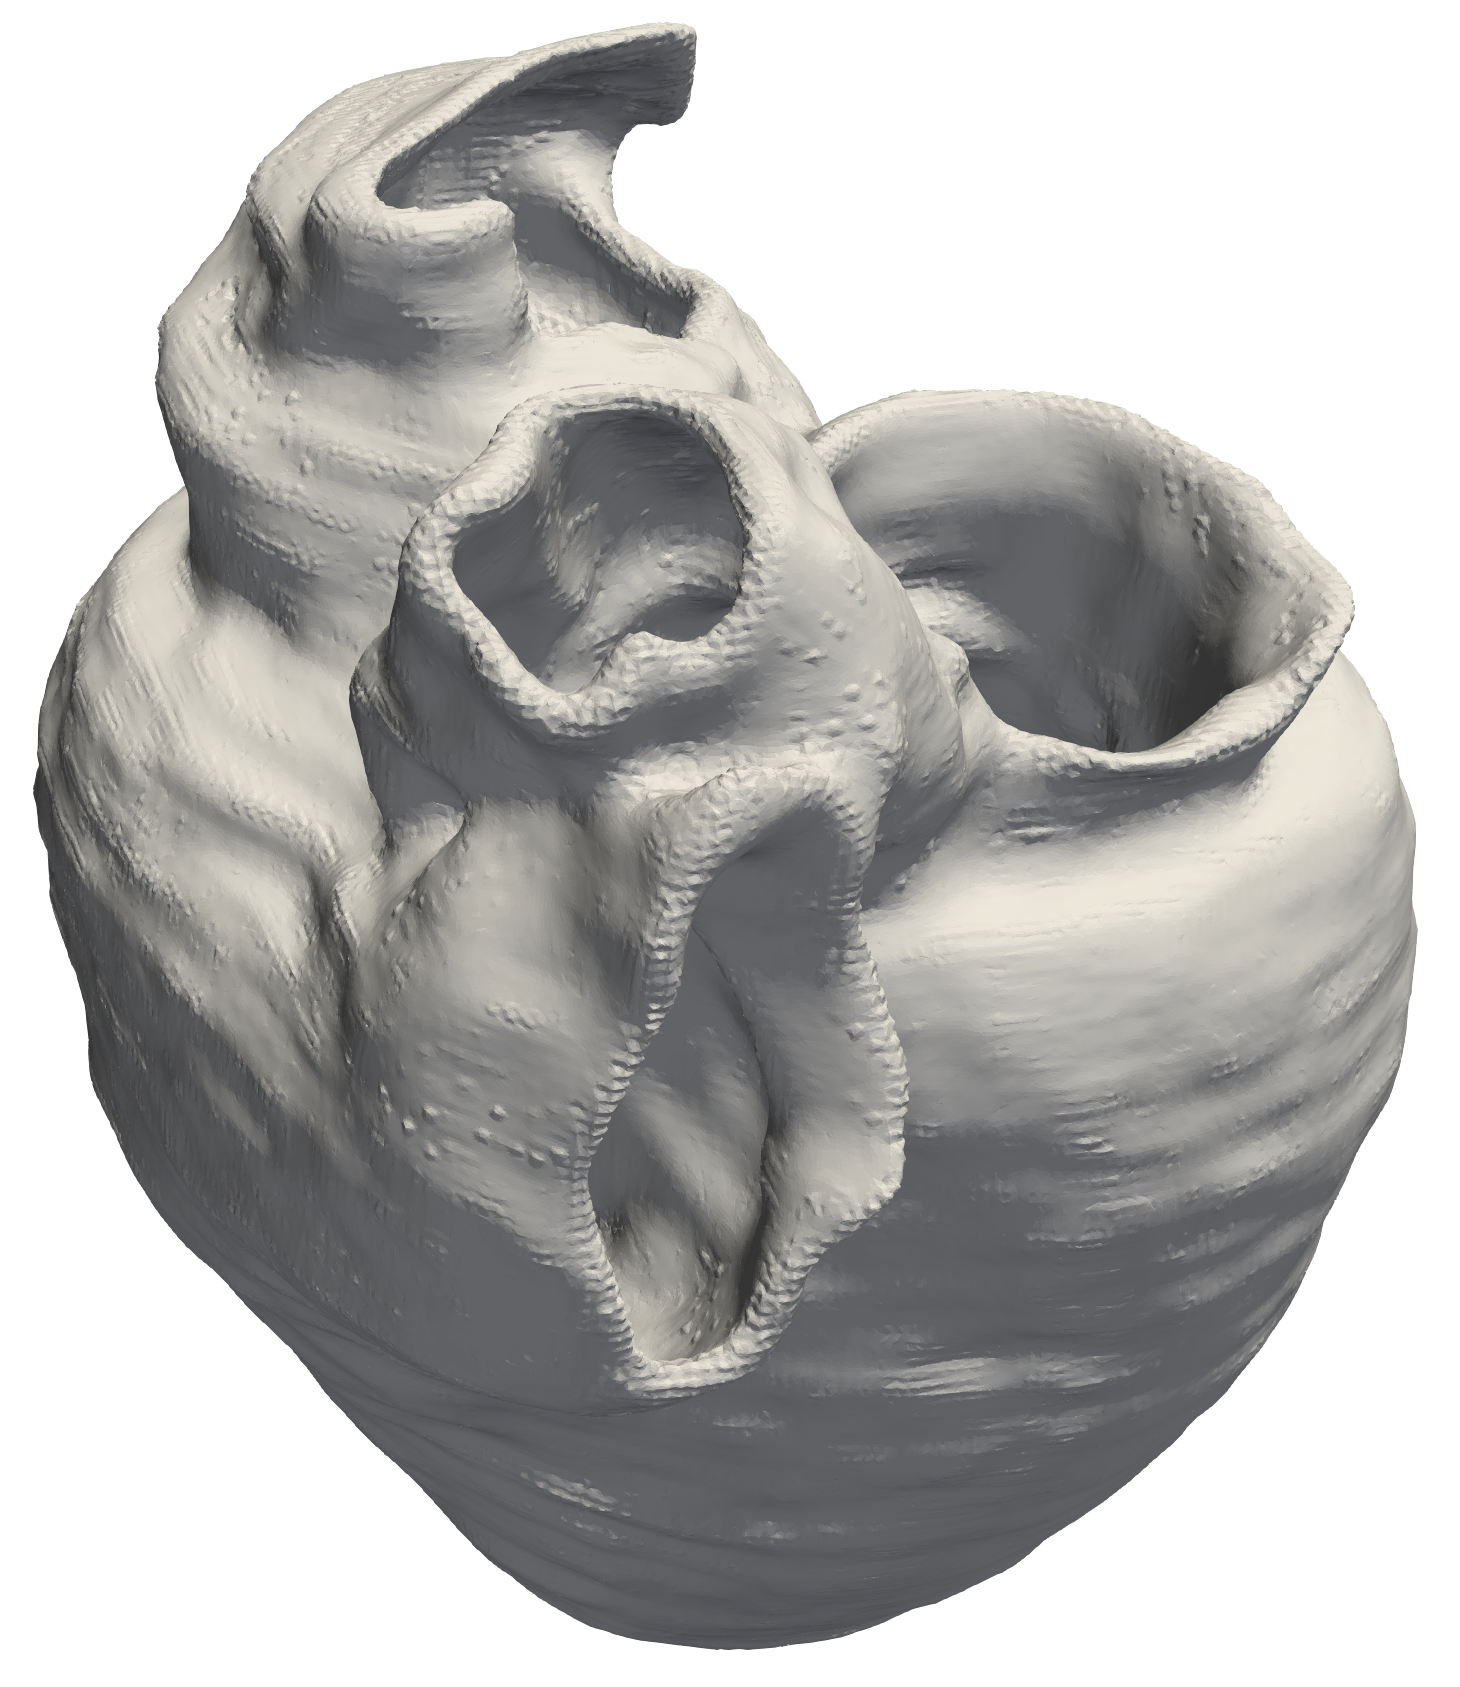
\includegraphics[scale=0.092]{media/2-shabaka/2-surf/4-finesurf.png}
\label{fig:shabakaseq4}}
\subfigure[]{%
		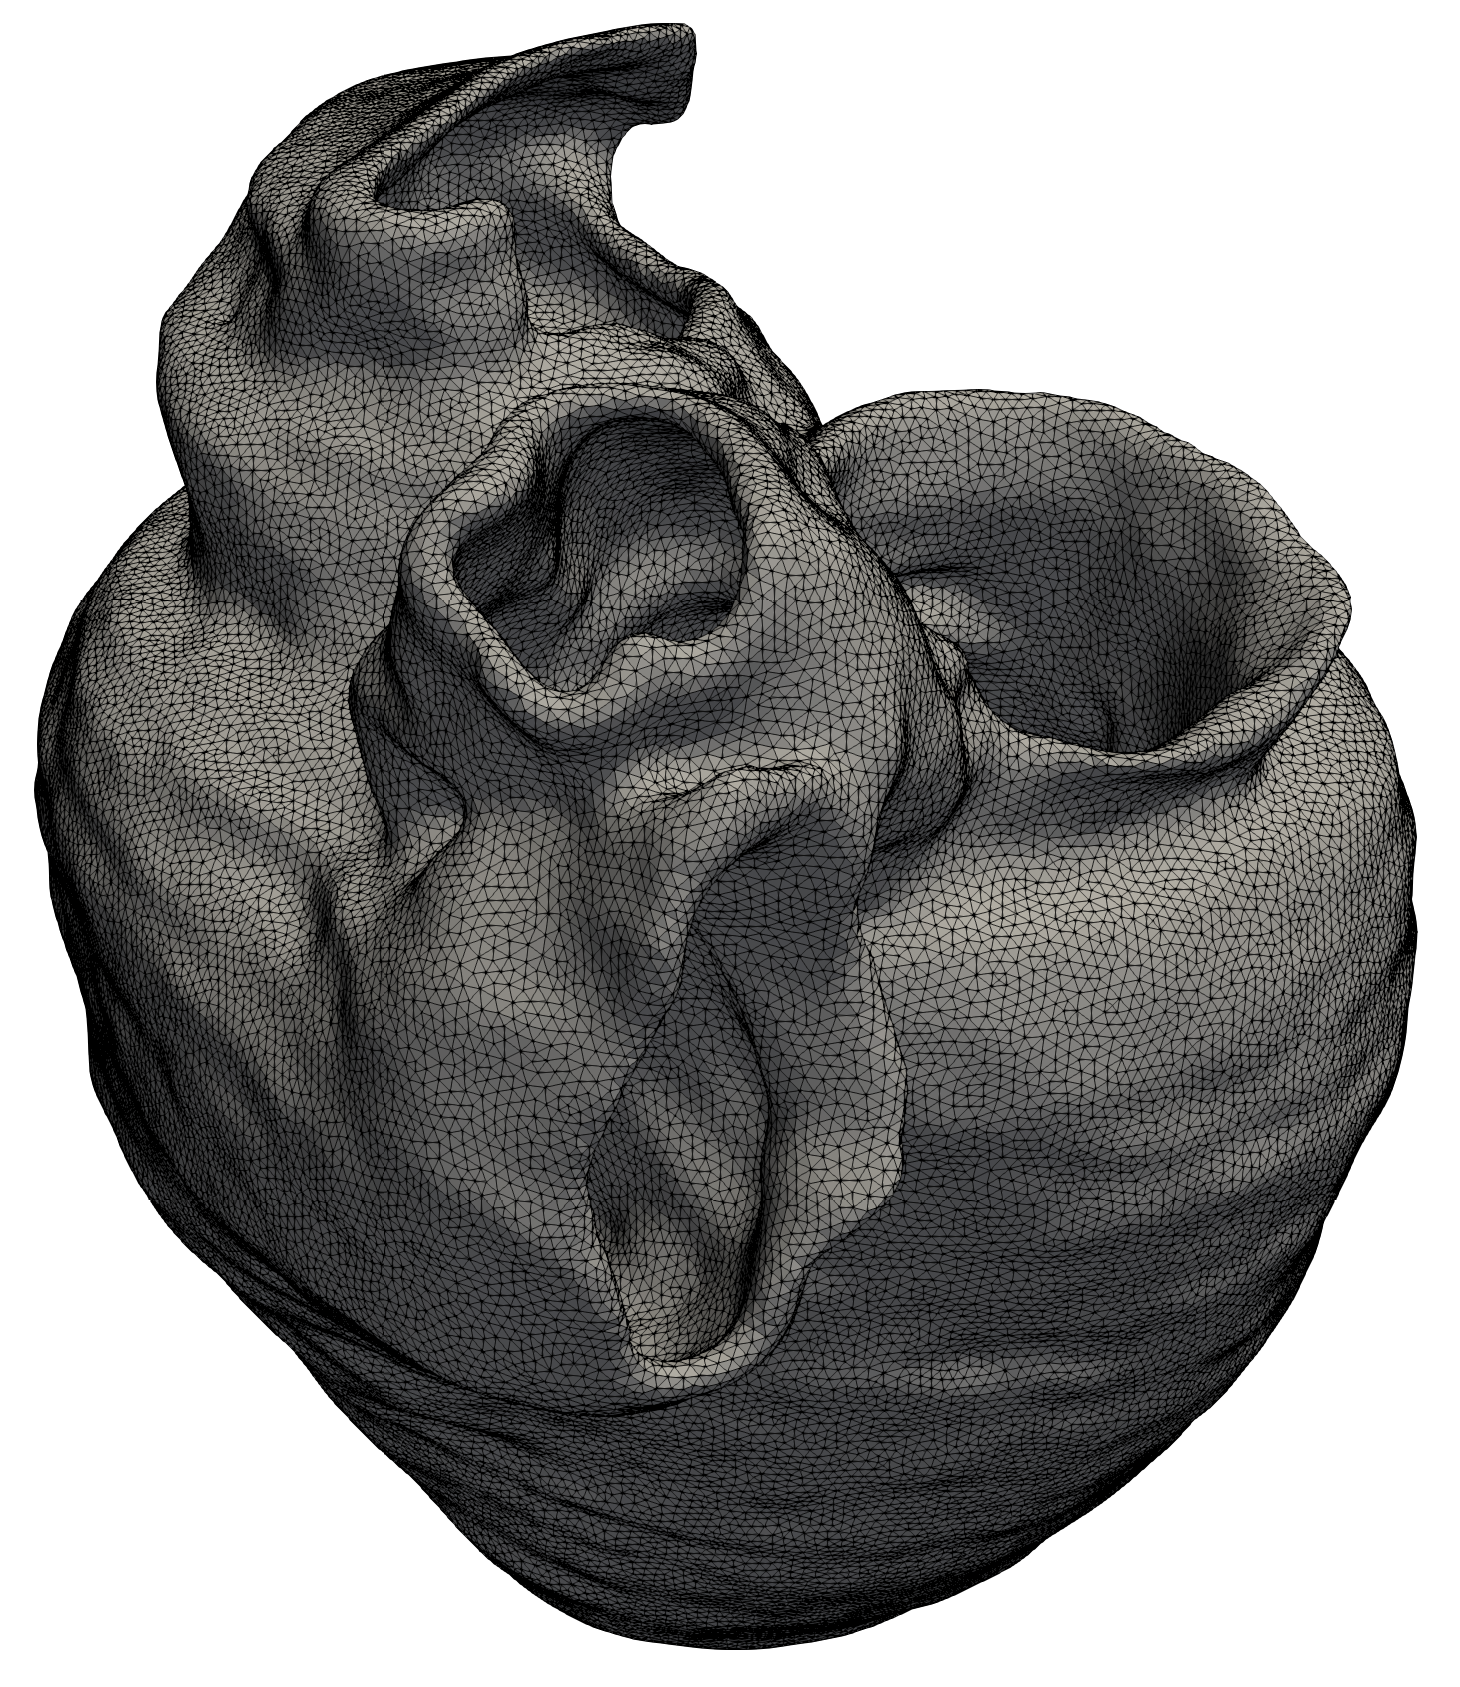
\includegraphics[scale=0.092]{media/2-shabaka/2-surf/5-surf.png}
\label{fig:shabakaseq5}}
%
\caption{(a) Segmented image, (b) point/normal placement, (c) oriented point cloud (normals not shown), c) cleaned surface mesh generated from Voronoi partition (edges not shown), and d) final decimated surface}
\label{fig:shabakaseq}
\end{figure}

\begin{figure}[ht!]
\centering
\vspace{2.5mm}
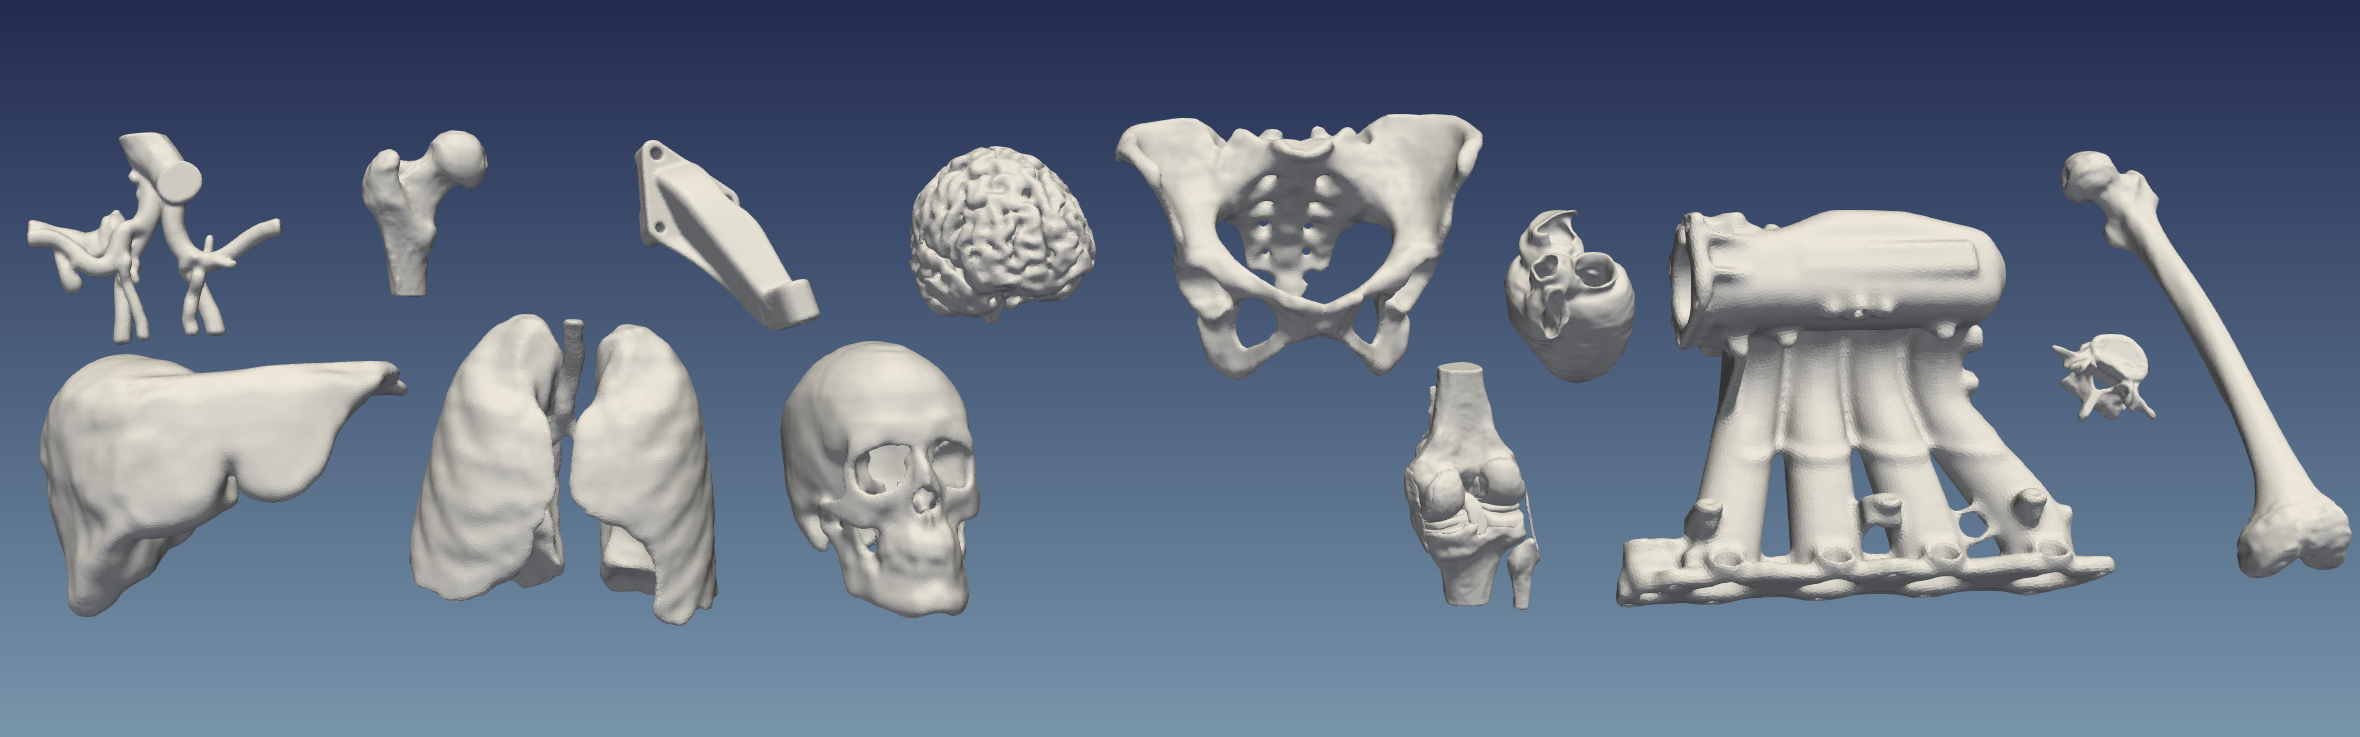
\includegraphics[width=1.0\textwidth]{media/2-shabaka/2-surf/6-showcase.png}
\caption{Suite of example surfaces generated from image data.}
\label{fig:showcase}
\end{figure}

\begin{figure}[ht!]
\centering
\vspace{2.5mm}
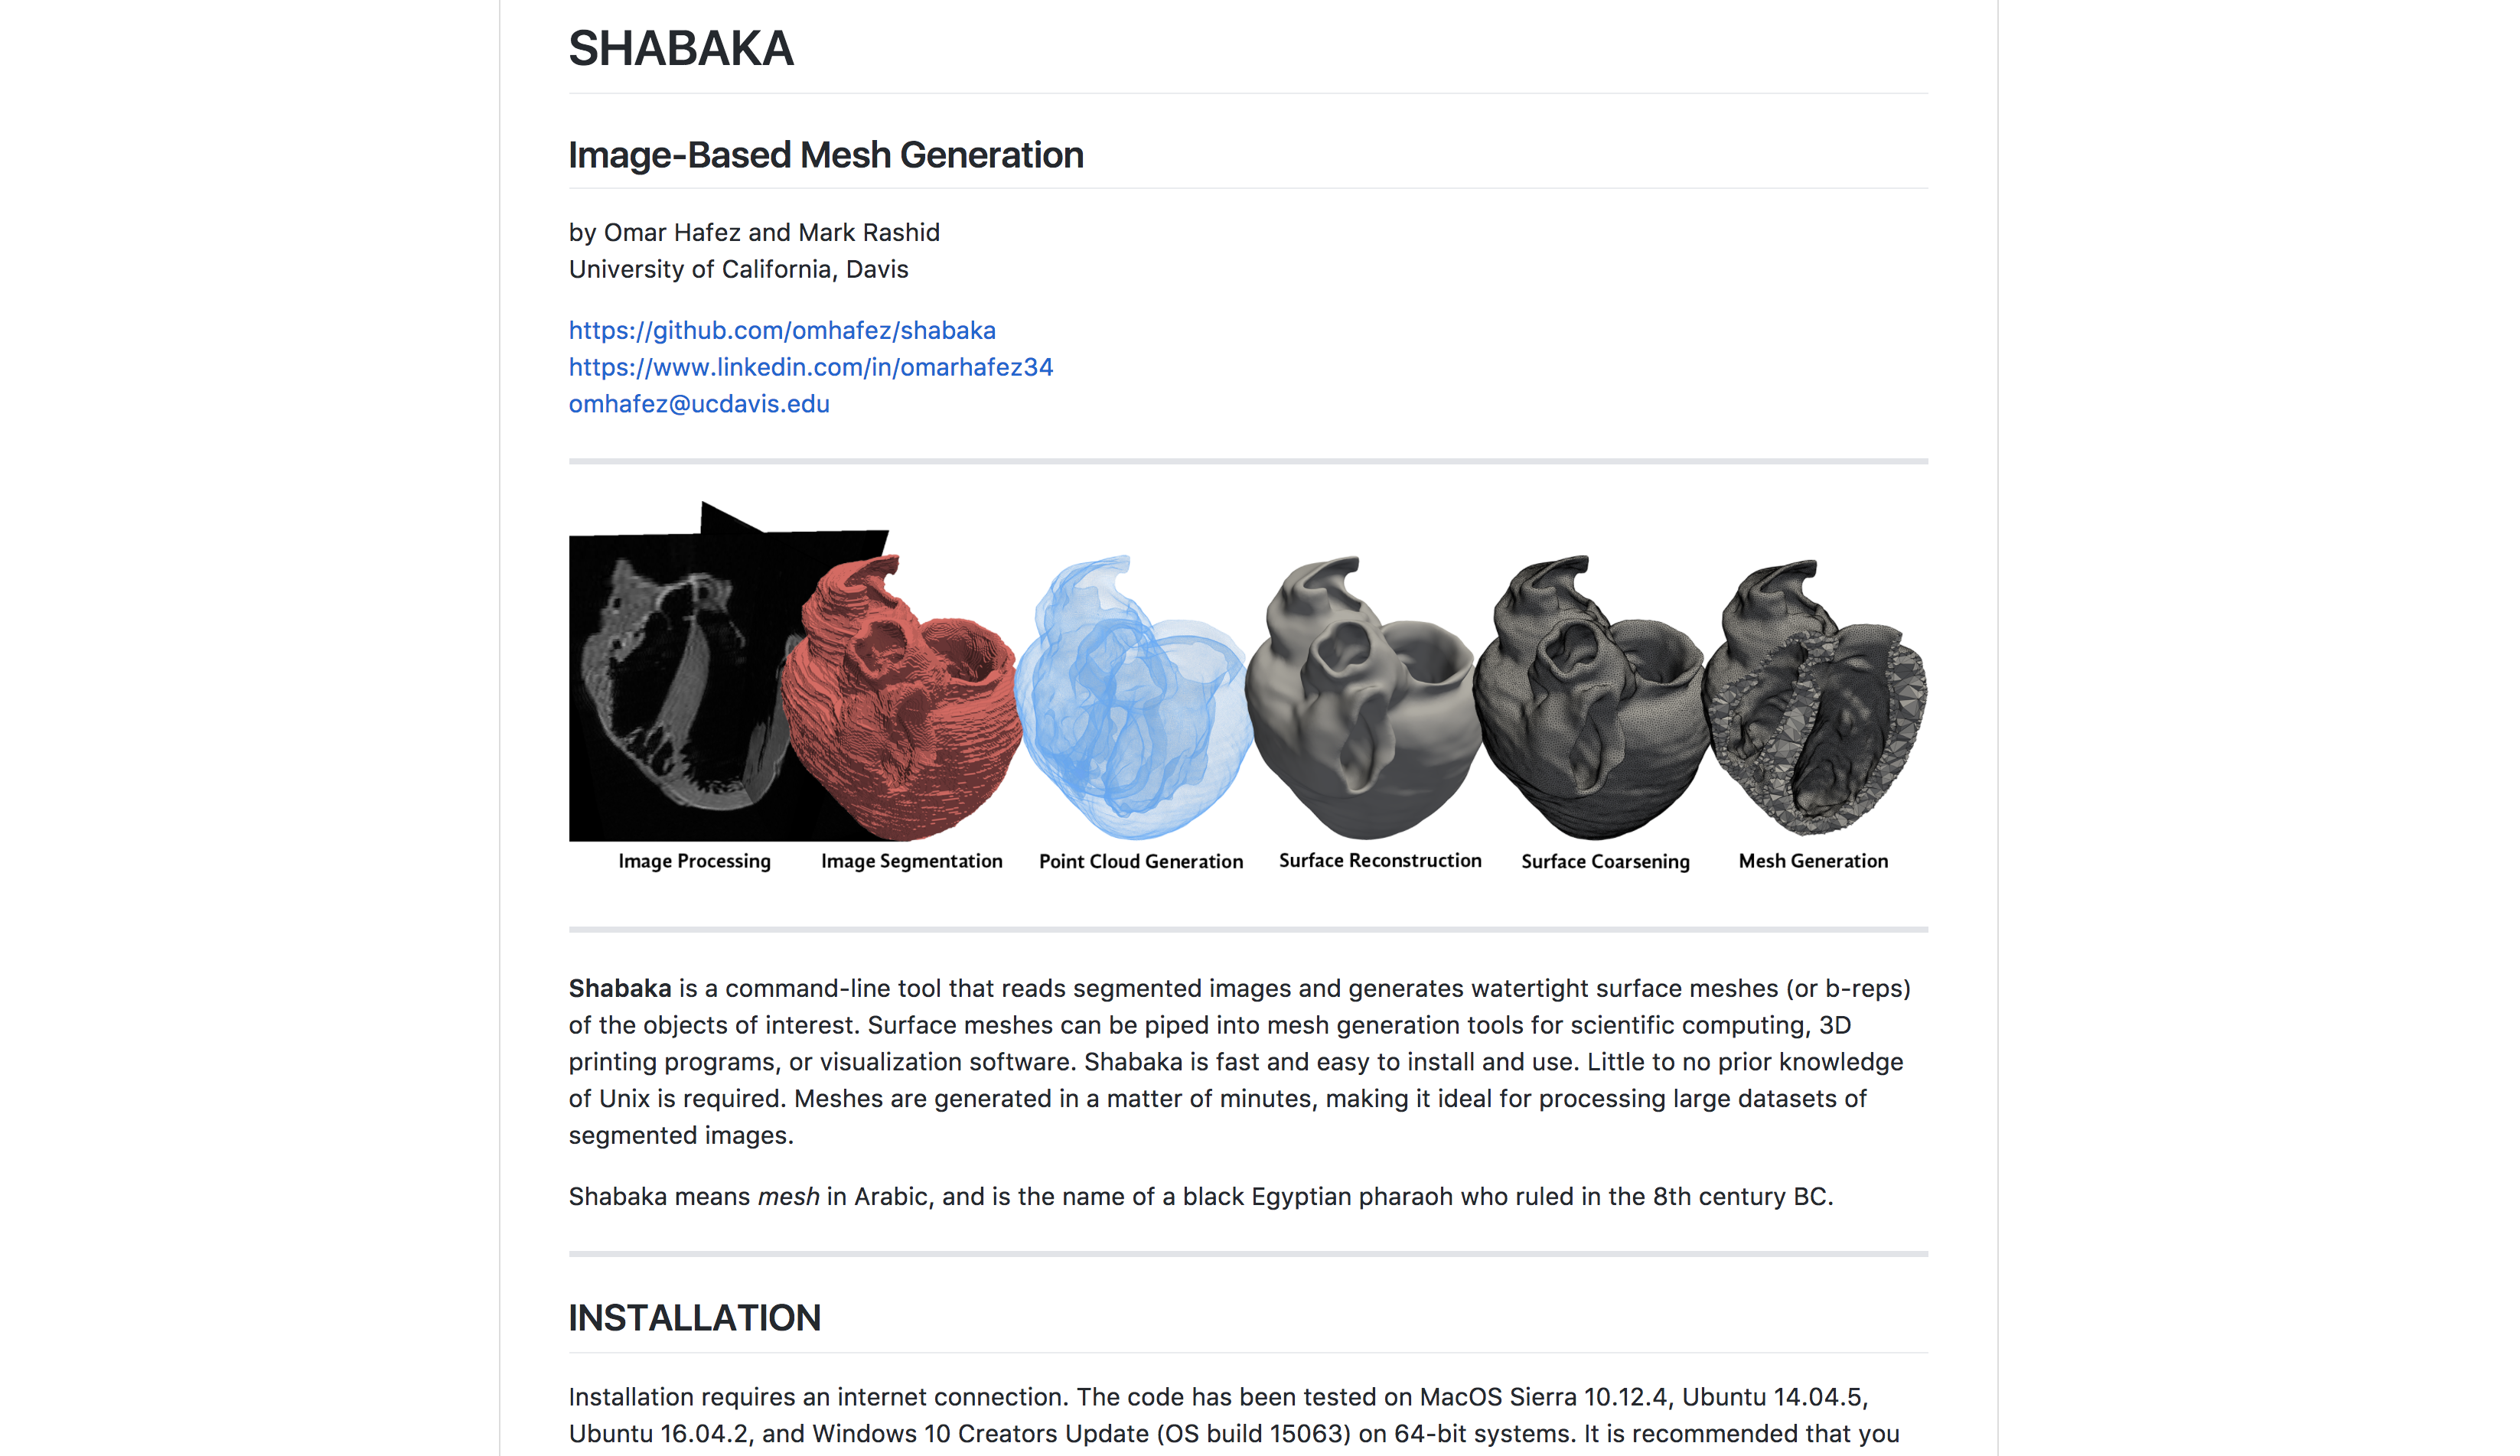
\includegraphics[width=1.0\textwidth]{media/2-shabaka/2-surf/7-shabaka.png}
\caption{Screenshot of Github repo}
\label{fig:github}
\end{figure}

%%%%%%%%%%%%%%%%%%%%%%%%%%%%%%%%%%%%%%%%%%%%%%%
%%%%%%%%%%%%%%%%%%%%%%%%%%%%%%%%%%%%%%%%%%%%%%%
\section{File Formats}
\label{File Formats-SURF}